\documentclass[a4paper, 12pt]{article}

\usepackage[warn]{mathtext} % Русский текст в формулах

\usepackage{tablefootnote}  % Cноски для таблиц

%Абзацный отступ

\usepackage{indentfirst}

%Рисунки

\usepackage{graphicx}
\usepackage{wrapfig}

%Гиперссылки и работа с цветом

\usepackage{hyperref}
\usepackage[rgb]{xcolor}
\hypersetup{			%Гиперссылки
	colorlinks=true, 	%false: ссылки в рамках
	urlcolor=blue		%на URL
}

%Русский язык

\usepackage[T2A]{fontenc}		%кодировка
\usepackage[utf8]{inputenc}		%кодировка исходного текста
\usepackage[english, russian]{babel}	%локализация и переносы


%Математика

\usepackage{amsmath, amsfonts, amssymb, amsthm, mathtools, mathrsfs}

%Пакет с градусом

\usepackage{gensymb}

%subfloat
\usepackage{subfig}

\author{Штрайх Роберт}
\title{Работа 4.3.1. Изучение дифракции света}
\date{09 апреля 2022 г.}

\begin{document}
\begin{titlepage}
	\centering
	\vspace{5cm}
	{\scshape\LARGE Московский физико-технический институт \par}
	\vspace{4cm}
	{\scshape\Large Лабораторная работа №4.3.1 \par}
	\vspace{1cm}
	{\huge\bfseries Изучение дифракции света\par}
	\vspace{1cm}
	\vfill
\begin{flushright}
  {\Large выполнили студенты 006 и 007 группы ФЭФМ}\par
	\vspace{0.3cm}
	{\Large Штрайх Роберт}\par
	\vspace{0.3cm}
	{\Large Петрова Софья}
\end{flushright}


	\vfill

% Bottom of the page
	Долгопрудный, 2022 г.
\end{titlepage}

\newpage

\textbf{Цель работы:} исследовать явления дифракции Френеля и Фраунгофера на щели, изучить влияние дифракции на разрешающую способность оптических инструментов.

\textbf{В работы используются:} оптическая скамья, ртутная лампа, монохроматор, щели с регулируемой шириной, рамка с вертикальной нитью, двойная щель, микроскоп на поперечных салазках с микрометрическим винтом, зрительная труба.

\section{Теоретические сведения и схема установки}
\subsection{Дифракция Френеля на щели}

Схема установки для наблюдения дифракции Френеля представлена на рис. 1. Световые лучи освещают щель~$S_2$ и испытывают на ней дифракцию. Дифракционная картина рассматривается с помощью микроскопа~М, сфокусированного на некоторую плоскость наблюдения~П.
		\begin{figure}[h]
		\begin{center}
			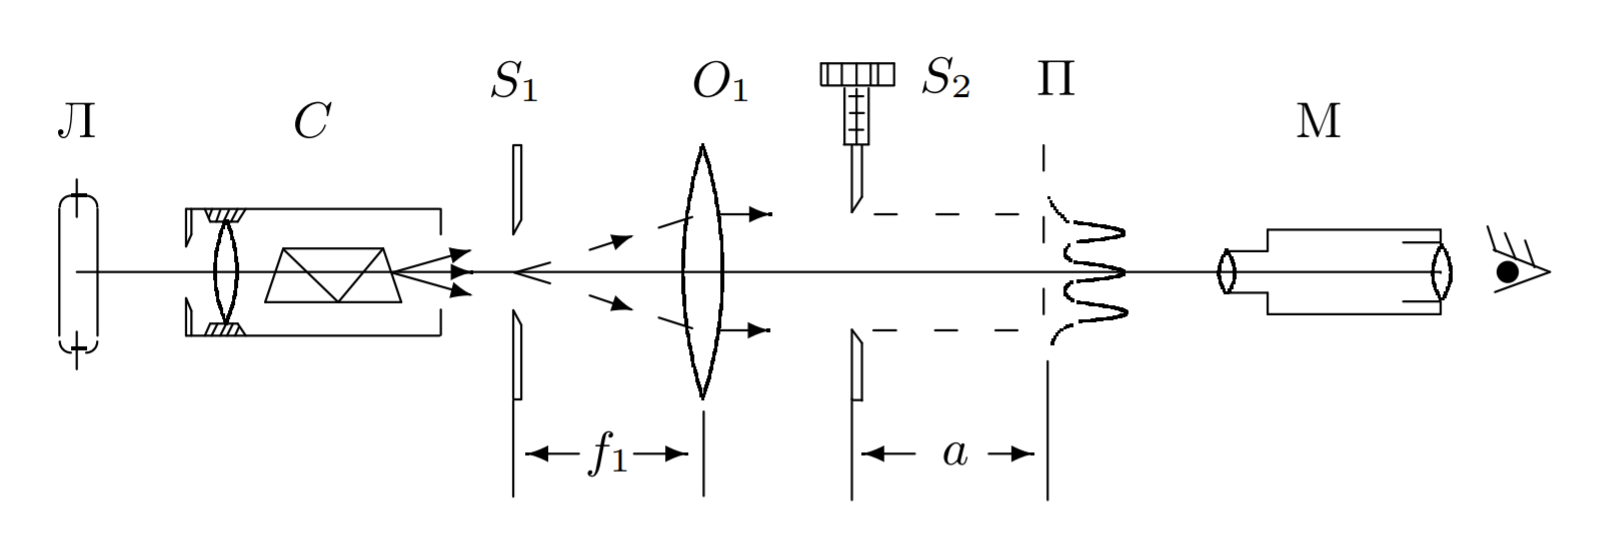
\includegraphics[width = 0.7\textwidth]{431-1.png}
			\caption{Схема установки для наблюдения дифракции Френеля}
		\end{center}
	\end{figure}

	Щель~$S_2$ освещается параллельным пучком монохроматического света с помощью коллиматора, образованного объективом~$O_1$ и щелью~$S_1$, находящейся в его фокусе. На щель~$S_1$ сфокусировано изображение спектральной линии, выделенной из спектра ртутной лампы~Л при помощи простого монохроматора~C.


	Распределение интенсивности света в плоскости наблюдения~П проще всего рассчитывать с помощью зон Френеля (для щели их иногда называют зонами Шустера). При освещении щели~$S_2$ параллельным пучком лучей (плоская волна) зоны Френеля представляют собой полоски, параллельные краям щели (рис. 2). Результирующая амплитуда в точке наблюдения определяется суперпозицией колебаний от тех зон Френеля, которые не перекрыты створками щели. Графическое определение результирующей амплитуды производится с помощью векторной диаграммы --- спирали Корню. Суммарная ширина $m$ зон Френеля $\xi_m$ определяется соотношением
	\begin{equation}
		\label{Ширина зон}
	\xi_m=\sqrt{zm\lambda},
	\end{equation}
	где $a$ --- расстояние от щели до плоскости наблюдения (рис. 1), а $\lambda$ --- длина волны.

	Вид наблюдаемой дифракционной картины определяется числом Френеля $C$:
	\begin{equation}
		C = \dfrac{b^2}{z \lambda} = \dfrac{1}{p^2}.
		\label{Число Френеля}
	\end{equation}
	Дифракционная картина отсутствует, когда плоскость наблюдения~П совпадает с плоскостью щели: при $C \rightarrow \infty$ мы имеем дело с геометрической оптикой. При небольшом удалении от щели, когда число Френеля $C \gg 1$ (на щели укладывается огромное число зон), дифракционная картина наблюдается только в узкой области на границе света и тени у краёв экрана.

	При последующем небольшом удалении от щели (или изменении ширины щели $S_2$) эти две группы дифракционных полос перемещаются практически независимо друг от друга. При дальнейшем увеличении расстояния (или уменьшении ширины щели~$S_2$) обе системы дифракционных полос постепенно сближаются и, наконец, при $C \gtrsim 1$ накладываются друг на друга. Распределение интенсивности в плоскости наблюдения в этом случае определяется числом зон Френеля, укладывающихся на полуширине щели. Если это число равно $m$, то в поле зрения наблюдается $n=m-1$ тёмных полос. Таким образом, по виду дифракционной картины можно оценить число зон Френеля на полуширине щели.

	\subsection{Дифракция Фраунгофера на щели}
	\begin{wrapfigure}{r}{0.5\textwidth}
		\begin{center}
			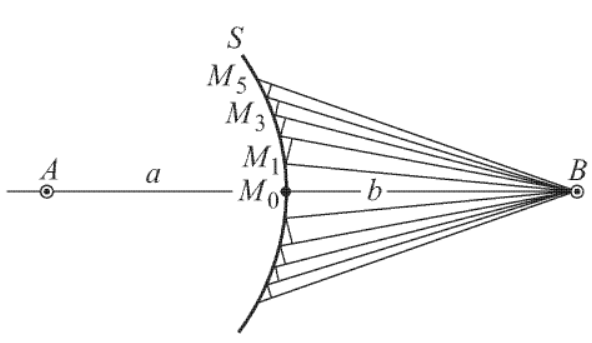
\includegraphics[width = 0.4\textwidth]{431-2.png}
		\end{center}
		\caption{Построение зон Френеля}
	\end{wrapfigure}
	Принцип Гюйгенса-Френеля:\\
	\textit{Каждый элемент волнового фронта можно рассматривать как центр  вторичного возмущения, порождающего вторичные сферические волны, а результирующее световое поле  в каждой точке пространства будет определяться интерференцией этих волн.}\\
	Теперь рассмотрим первое применение этого принципа, получившее название \textit{метод зон Френеля}


	Для этого рассмотрим действие световой волны действующей из точки $A$ в какой-то точке $B$.
	В этом случае можно, взяв точку $M_0$ в качестве центра (см. рис. 1), построить ряд концентрических сфер, радиусы которых начинаются с $b$ и увеличиваются каждый раз на половину длины волны $\frac{\lambda}{2}$. При пересечении с плоским фронтом волны $F$ эти сферы дадут концентрические окружности. Таким образом, на фронте волны появятся кольцевые зоны (зоны Френеля) с радиусами $r_1, r_2$ и т. д.

	Из геометрических соображений посчитав, можно получить, что
	\begin{equation}
	r_i = i \sqrt{\lambda z}.
	\end{equation}
		\begin{wrapfigure}{r}{0.3\textwidth}
		\begin{center}
			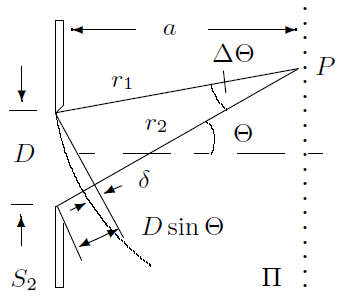
\includegraphics[width = 0.3\textwidth]{431-3.png}
		\end{center}
		\caption{К фазовым соотношениям при дифракции Фраунгофера}
	\end{wrapfigure}

	Картина дифракции упрощается, когда ширина щели становится значительно меньше ширины первой зоны Френеля, т.е. если
	\begin{equation}
	b \ll\sqrt{\lambda z}
	\end{equation}
	Это условие всегда выполняется при достаточно большом $a$. В этом случае говорят, что \textit{дифракция Фраунгофера}. Дифракционную картину в этом случае называются \textit{дифракцией Фраунгофера}. При выполнении пункта $(2)$ у нас упрощаются фазовые соотношения, что поясняет рис. 2, в итоге с хорошим приближением можно считать, что разность хода между крайними лучами, приходящими от щели в точке наблюдения $P$, с хорошим приближением равна
	\begin{equation}
	\Delta = r_2 - r_1 \approx b \sin \theta \approx b \cdot \theta
	\end{equation}
	Здесь предполагается, что $\theta$ достаточно мал.
	Дифракцию Фраунгофера можно наблюдать на установке рис. 1, но для удобства к подобной установке добавляется объектив $O_2$.

	\begin{figure}[h]
		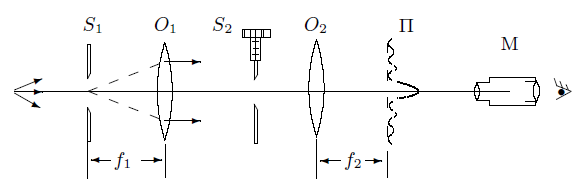
\includegraphics[width = 0.7\textwidth]{431-4.png}
		\centering
		\caption{Схема установки для наблюдения дифракции Фраунгофера}
		\label{Установка_Фраунгофер}
	\end{figure}
	Дифракционная картина здесь наблюдается в фокальной плоскости объектива $O_2$. Каждому значению $\theta$ соответствует в этой плоскости точка, отстоящая от оптической оси на расстоянии
	\begin{equation}
	X = f_2 \tg \theta \approx f_2 \theta.
	\end{equation}
	Объектив не вносит разности хода между интерферирующими лучам, поэтому в его фокальной плоскости наблюдается неискажённая дифракционная картина. При $\theta = 0$ разность хода между лучами нулевая, поэтому в центре поля зрения дифракционный максимум. Первый минимум соответствует $\theta_1$ такому, что в точке наблюдения разность хода пробегаем все значения от 0 до $2\pi$. Аналогично рассуждая, для $m$-й полосы
	\begin{equation}
	\theta_m = \frac{m \lambda}{b}
	\end{equation}
	Расстояние $X_m$ тёмной полосы от оптической оси из (5) и (6)
	\begin{equation}
		\label{Расстояние X_m}
	X_m = f_2m\frac{\lambda}{b}
	\end{equation}

	\subsection{Дифракция Фраунгофера для двух щелей}
	Для наблюдения дифракции Фраунгофера на двух щелях $S_2$ заменим экраном Э с двумя щелями. При этом для оценки влияния ширины входной щели на чёткость вместо $S_1$ поставим щель с микрометрическим винтом.
	\begin{figure}[h]
		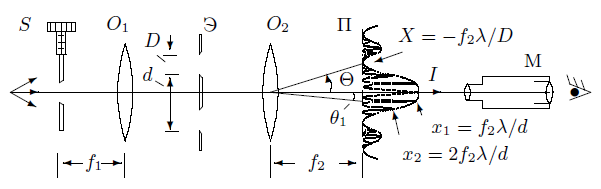
\includegraphics[width = 0.7\textwidth]{431-5.png}
		\centering
		\caption{Схема установки для наблюдения дифракции Фраунгофера на двух щелях}
	\end{figure}
	Два дифракционных изображения входной щели, одно из которых образовано лучами, прошедшими через левую, а другое -- через правую щели, накладываются друг на друга.
	Если входная щель достаточно узка, то дифракционная картина в плоскости П подобна той, что получалась при дифракции на одной щели, однако вся картинка испещерена рядом дополнительных узких полос, наличие которых объясняется суперпозицией световых волн через разные щели. Светлая интерфереционная полоса наблюдается в случаях, когда разность хода равна целому числу длин волн. Таким образом, угловая координата максимума порядка $m$ равна
	\begin{equation}
	\theta_m = \dfrac{m \lambda}{d},
	\end{equation}
	где $d$ -- расстояние между щелями. Отсюда расстояние между соседними интерфереционными полосами в плоскости П равно
	\begin{equation}
	\delta x = f_2 \dfrac{\lambda}{d}
	\end{equation}
	Число интерференционных полос укладывающихся в области центрального максимума равна отношению ширины главного максимума $\frac{2\lambda f_2}{b}$ к расстоянию между соседними полосами:
	\begin{equation}
	n = \dfrac{2\lambda f_2}{b} \dfrac{1}{\delta f}= \dfrac{2d}{b}.
	\end{equation}
	При дифракции света на двух щелях чёткая система интерференционных полос наблюдается только при достаточно узкой ширине входной щели $S$. При увеличении ширины картинка пропадает и появляется вновь, но полосы при этом сильно размыты и видны плохо.

	\subsection{Влияние дифракции на разрешающую способность оптического инструмента}
		\begin{figure}[h]
			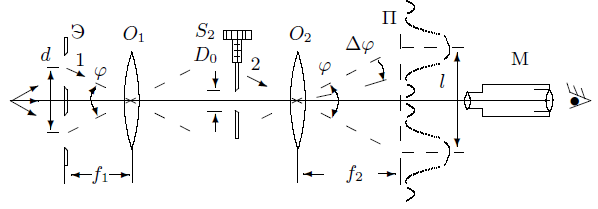
\includegraphics[width = 0.8\textwidth]{431-6.png}
			\centering
			\caption{Схема установки для исследования разрешающей способности оптического инструмента}
		\end{figure}
		В отсутствие щели $S_2$ линзы $O_1$ и $O_2$ создают на плоскости П изоюражение щели $S_1$ и это изображение рассматриваются микроскопом М. Таким образом, установку можно рассматривать как оптический инструмент, предназначенные для получения изображения предмета. Если перед $O_2$ расположить $S_2$, то изображение объекта будет искажено из-за дифракции. Чем меньше ширина щели, тем сильнее искажение. Качественной характеристикой этого искажения может служить $\varphi_{min}$ --- минимальное угловое расстояние между объектами (источниками), которые всё ещё воспринимаются как раздельные. Поместим вместо $S_1$ экран Э с двумя щелями с расстоянием $d$. Тогда на $S_2$ будут падать два пучка света с углом
		\begin{equation}
		\varphi = \dfrac{d}{f_1}
		\end{equation}
		Из геометрии расстояние $l$ между изображениями щелей в плоскости П равно
		\begin{equation}
		l = \varphi f_2 = d \dfrac{f_2}{f_1}.
		\end{equation}
		Ширина $\Delta \varphi$ определяется дифракцией на $S_2$. Условия, при которых изображения различимы разные для разных наблюдателей, поэтому используют \textit{критерий Рэлея} -- \textit{максимум одного дифракционного пятна должен совпадать с минимумом другого}. В наших условиях это значит, что угловая полуширина $\frac{\lambda}{b}$ равна угловому расстоянию $\frac{l}{f_2}$.

\section{Ход работы}
\subsection{Дифракция Френеля}

\begin{enumerate}
	\item Добьемся наибольшей четкости дифракционной картины и найдем резкое изображение щели (четкие края без дифракционных полос). Положение микроскопа $x_0 = $ 68,9 см.

	\item Передвигая микроскоп, снимем зависимость числа $n$ наблюдаемых полос от расстояния микроскопа до плоскости наблюдения $z$.
	\begin{center}
		\begin{tabular}{|c|c|c|c|c|c|}
			\hline
			$n$ & 1    & 2    & 3    & 4    & 5    \\ \hline
			$z$, мм & 24 & 17 & 13 & 10 & 8 \\ \hline
		\end{tabular}
	\end{center}

\clearpage
\begin{figure}[h!]
\begin{minipage}{0.5\textwidth}
	\center{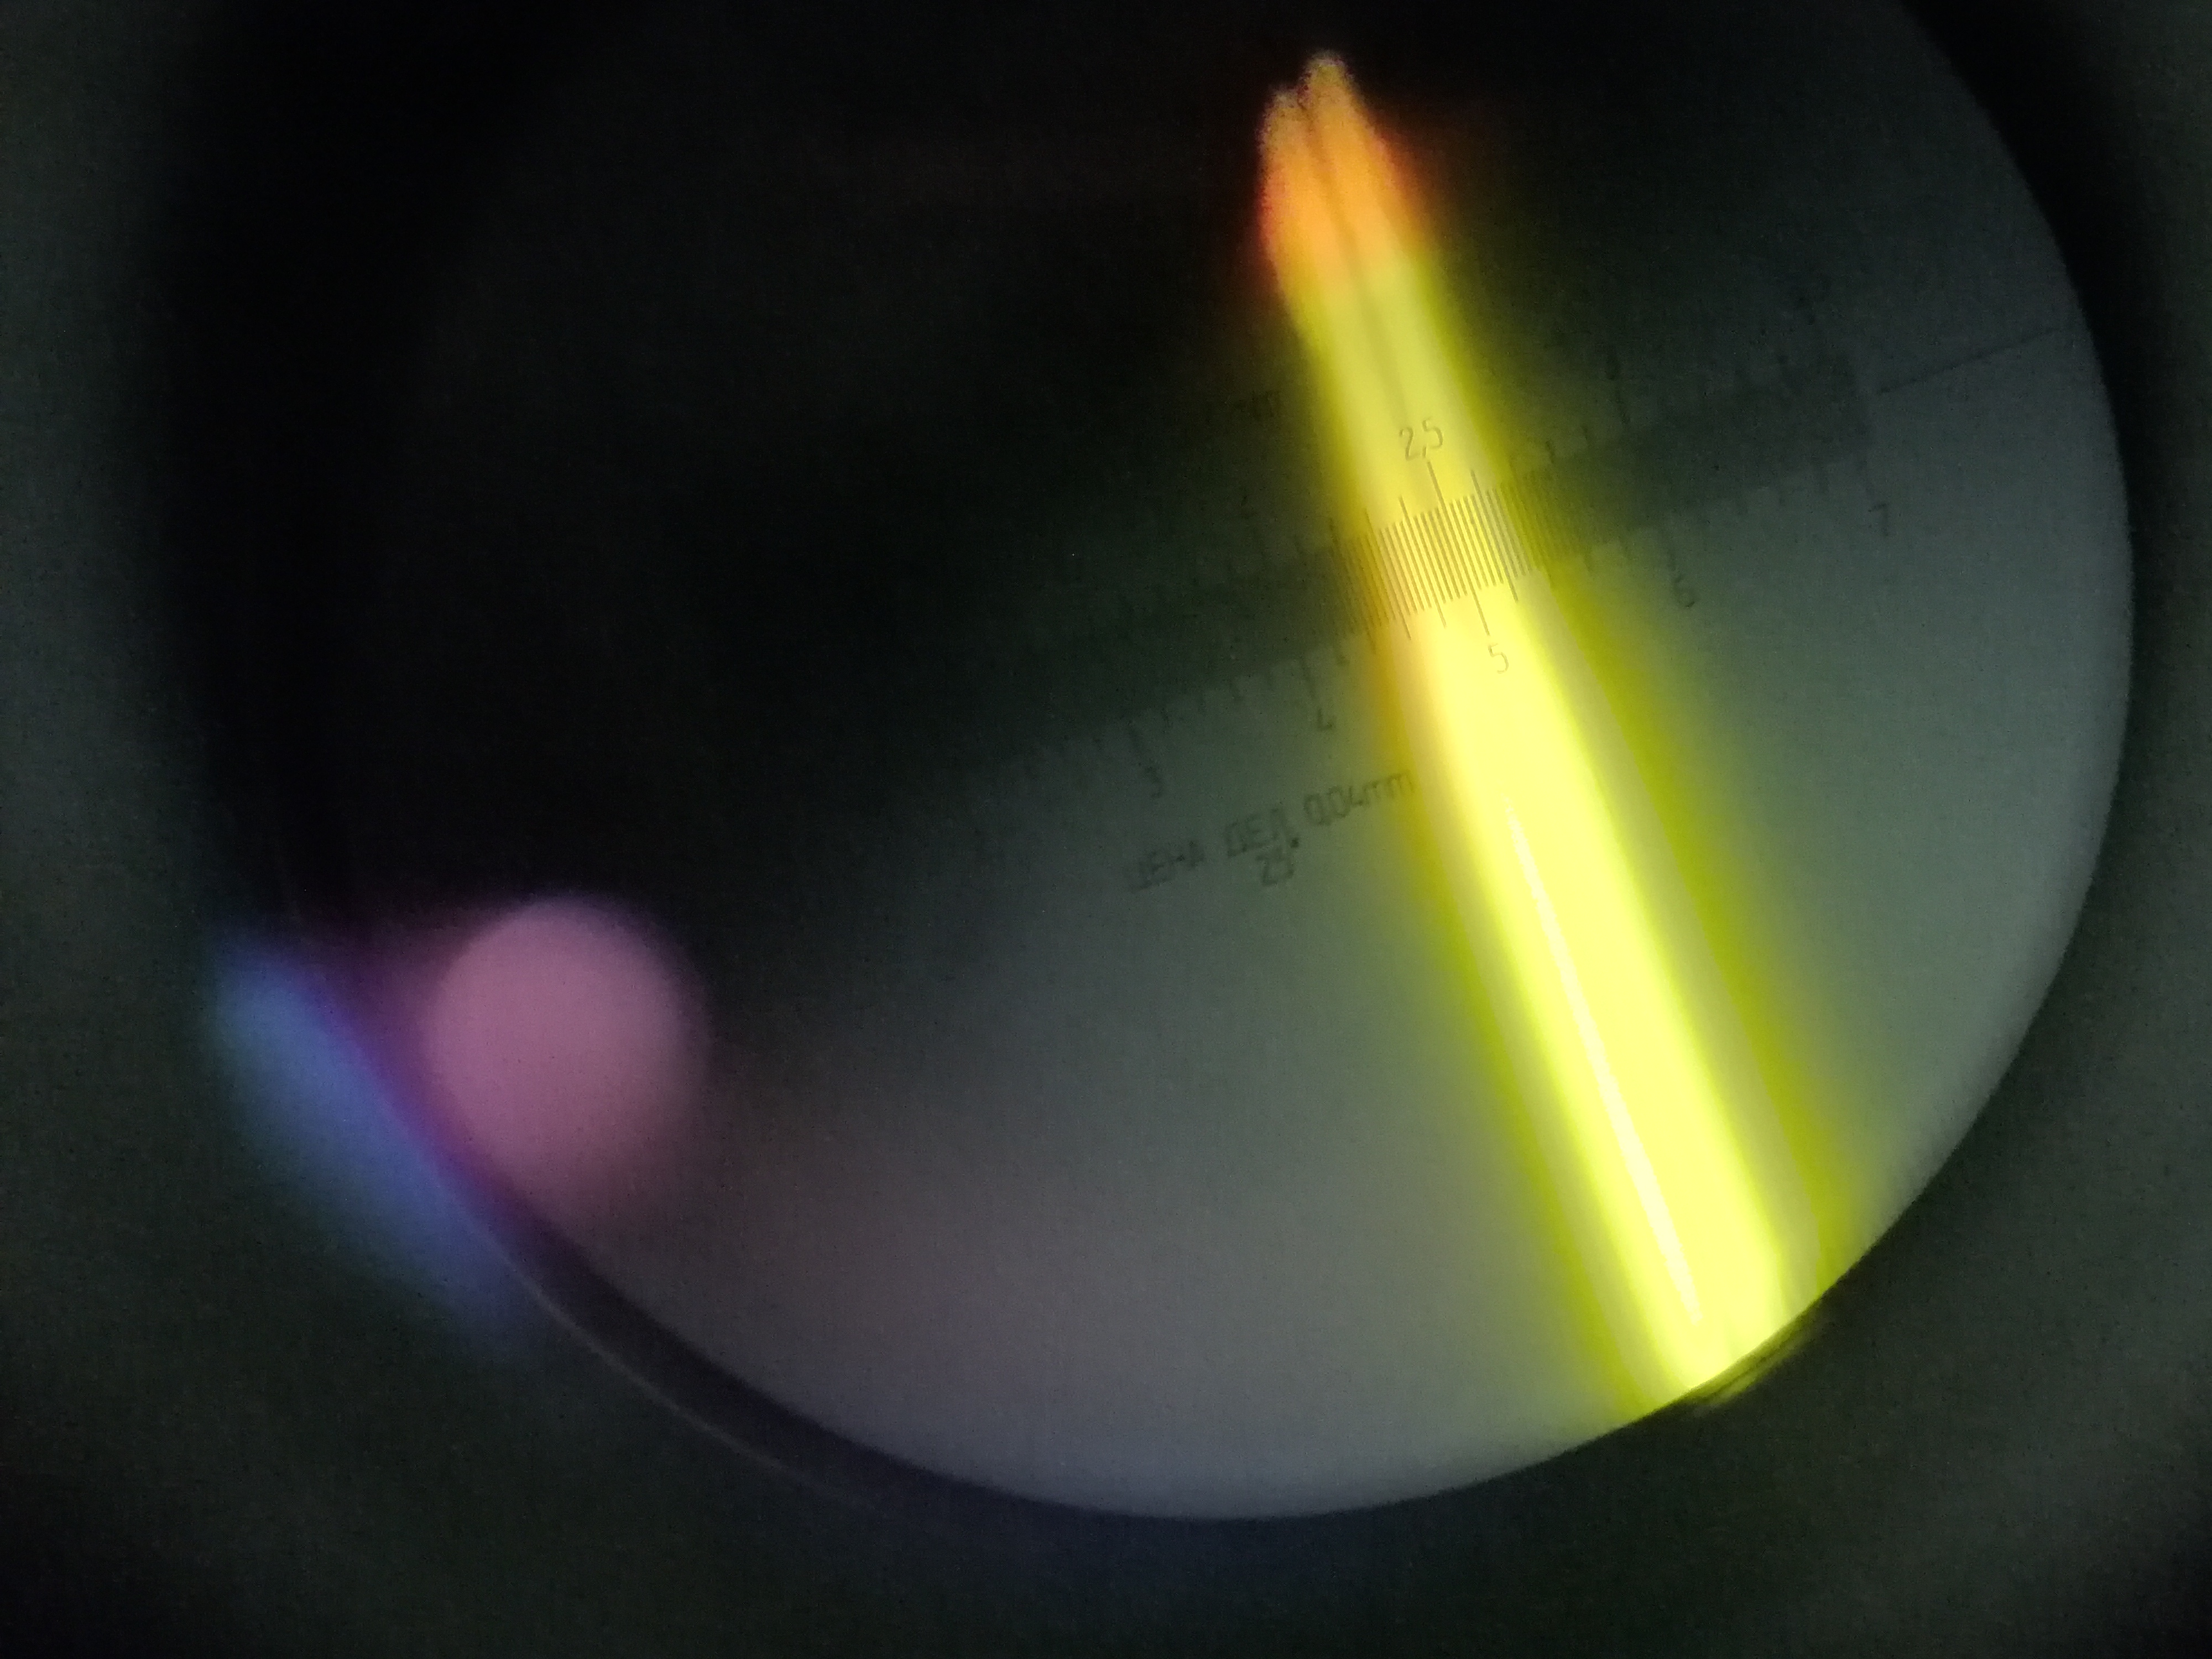
\includegraphics[width=1\textwidth]{frenel-1.jpg} \\ а) 1 полоса}
\end{minipage}
\begin{minipage}{0.5\textwidth}
	\center{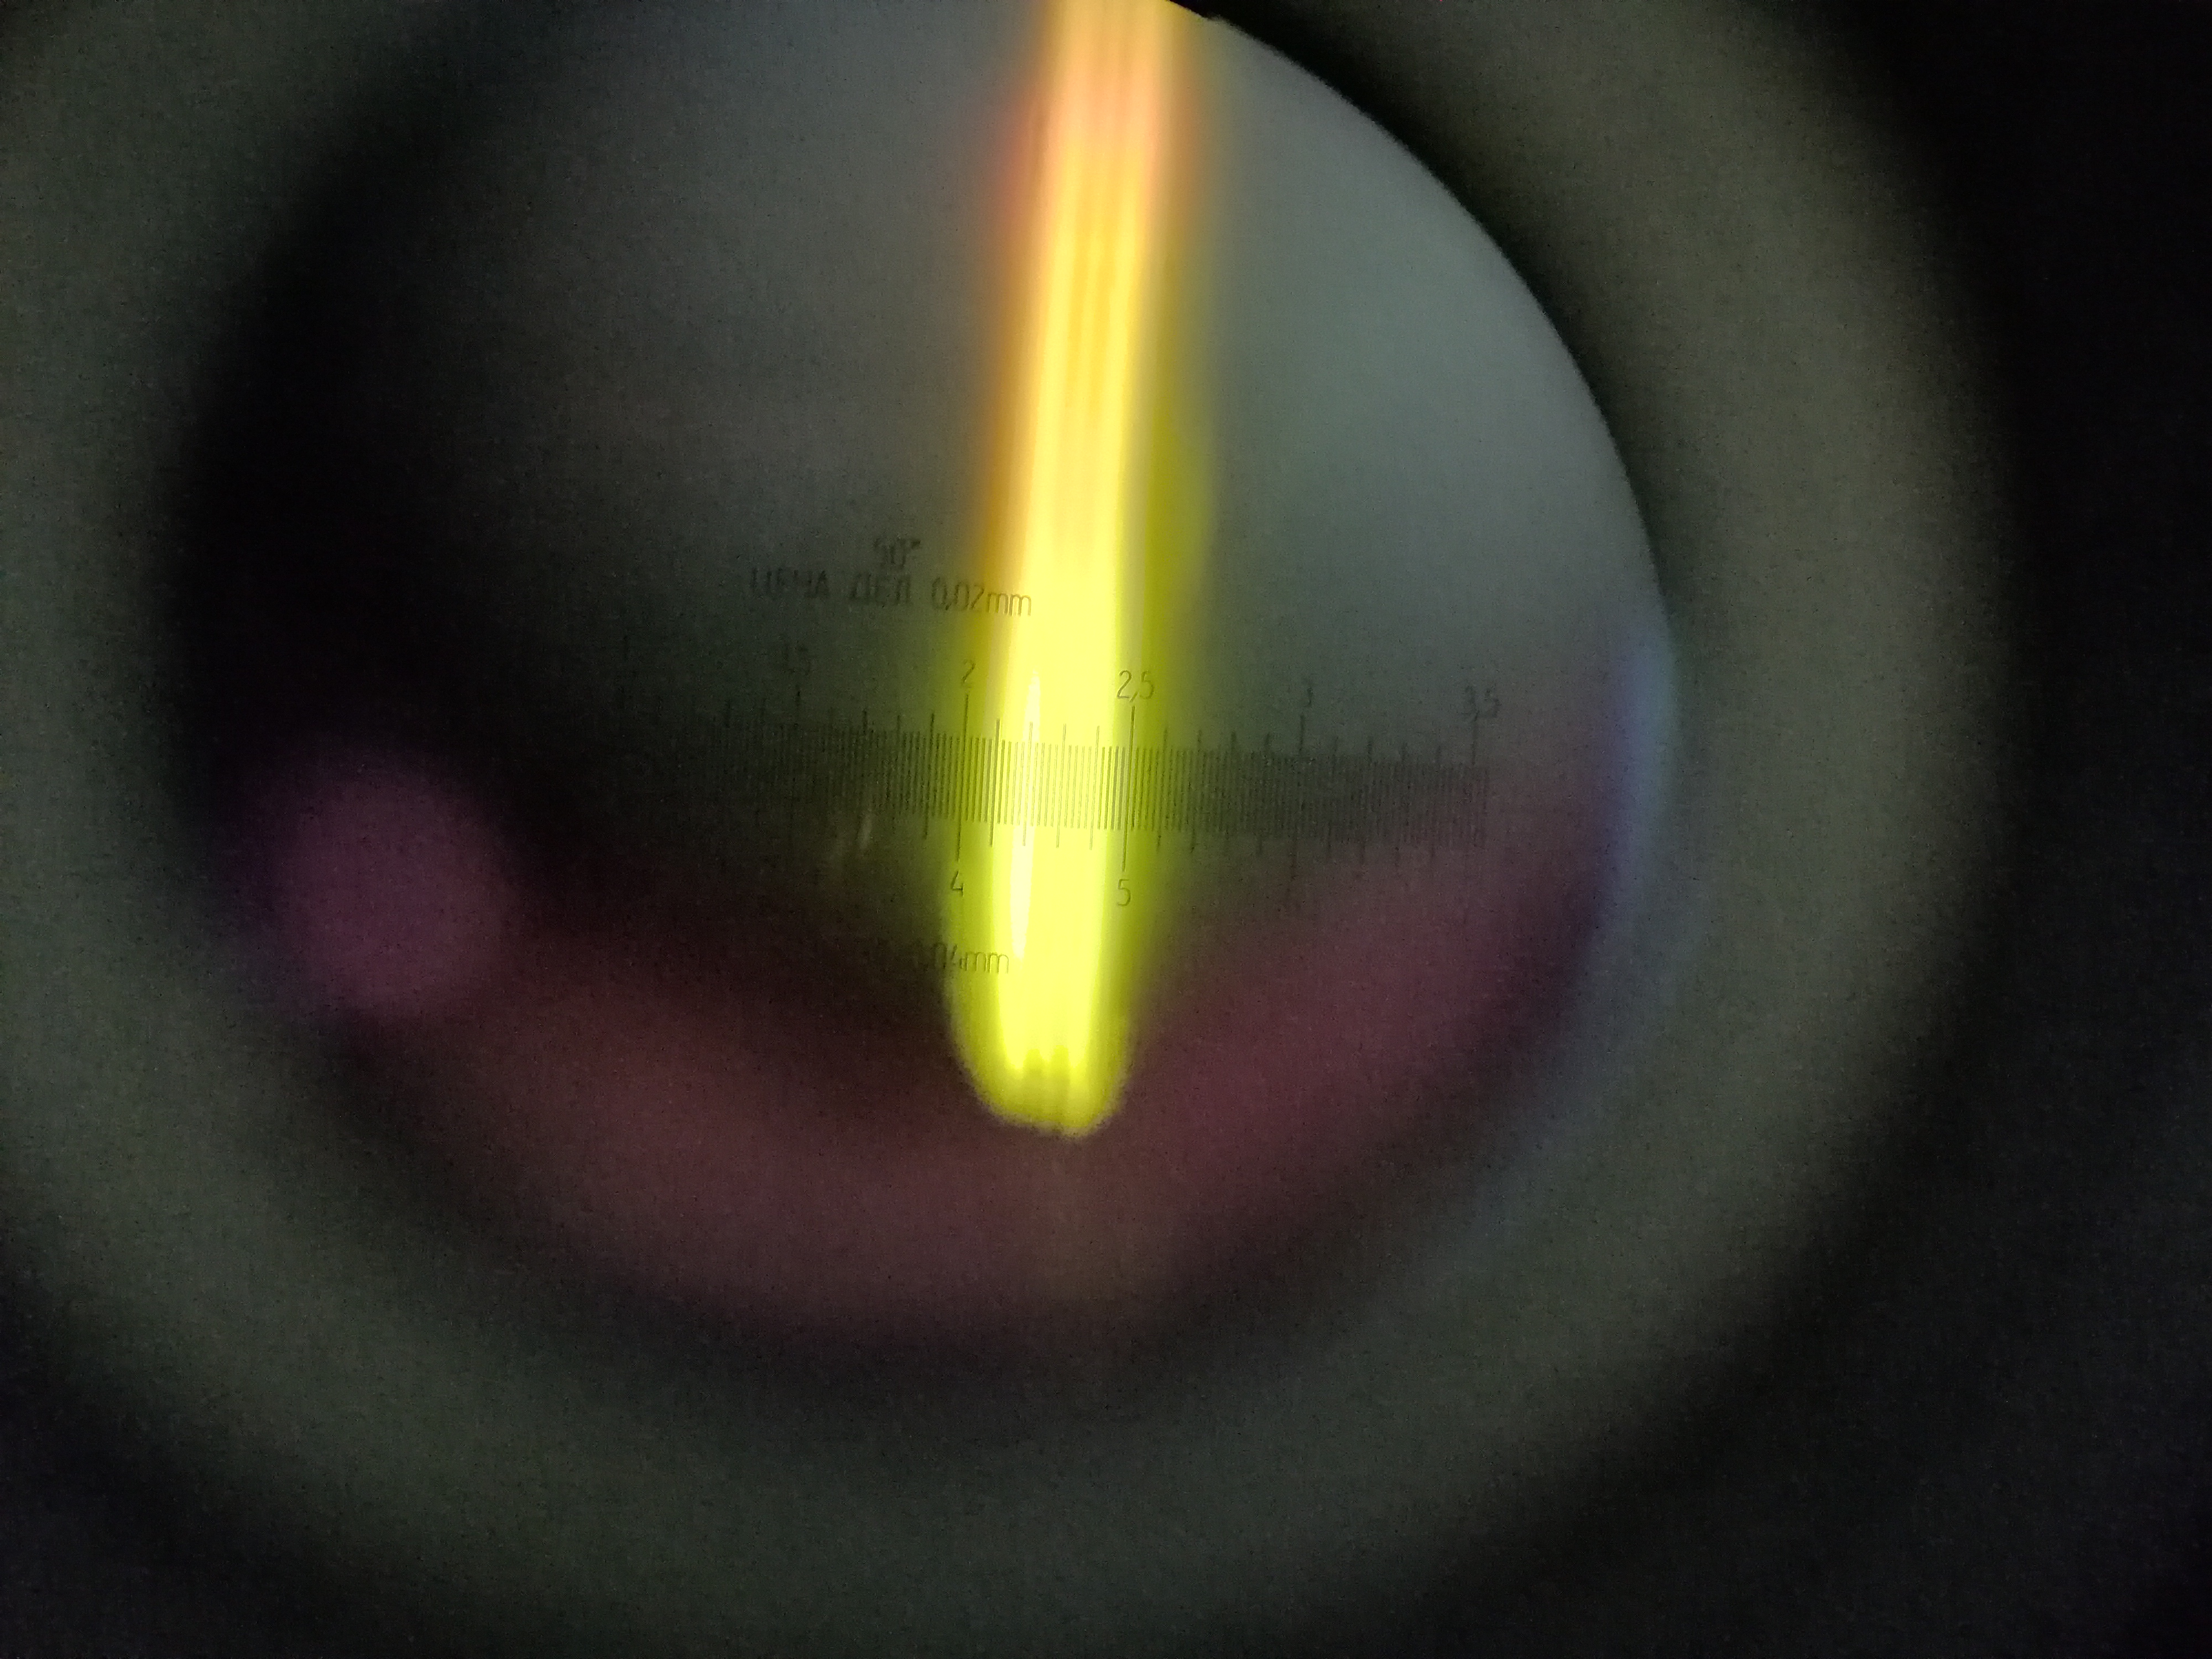
\includegraphics[width=1\textwidth]{frenel-2.jpg} \\ б) 2 полосы}
\end{minipage}
\begin{minipage}{0.5\textwidth}
	\center{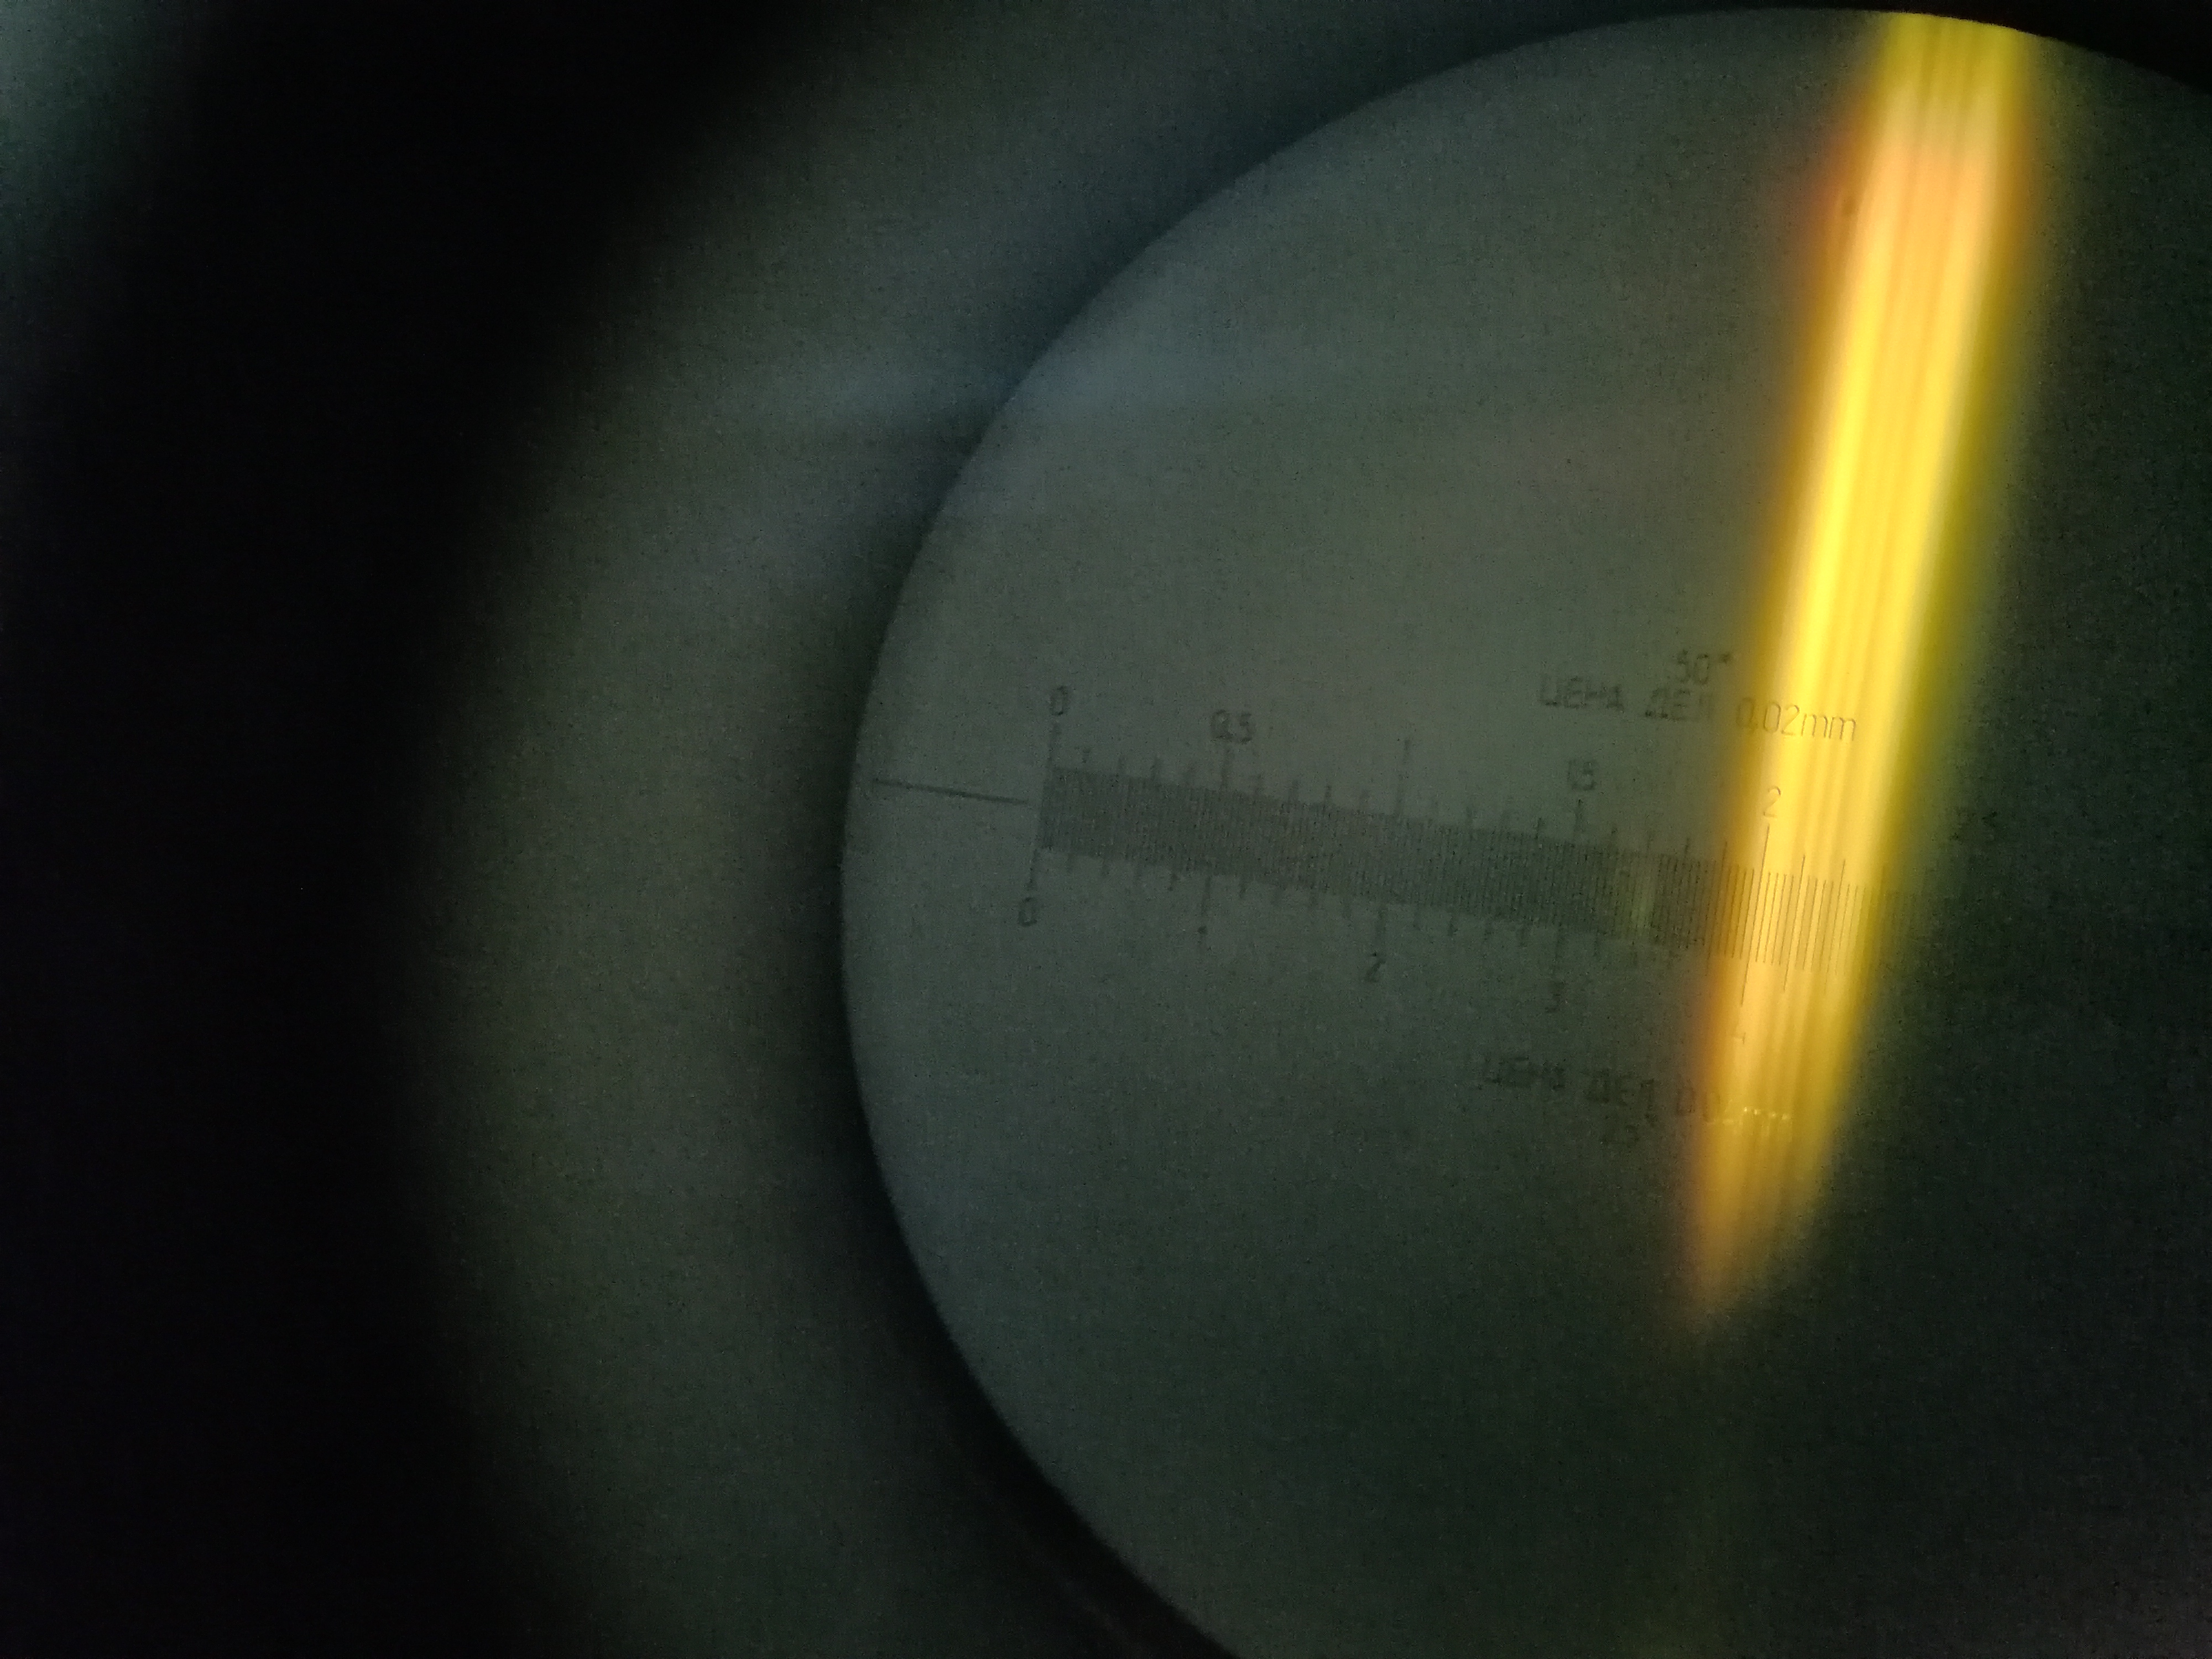
\includegraphics[width=1\textwidth]{frenel-3.jpg} \\ в) 3 полосы}
\end{minipage}
\begin{minipage}{0.5\textwidth}
	\center{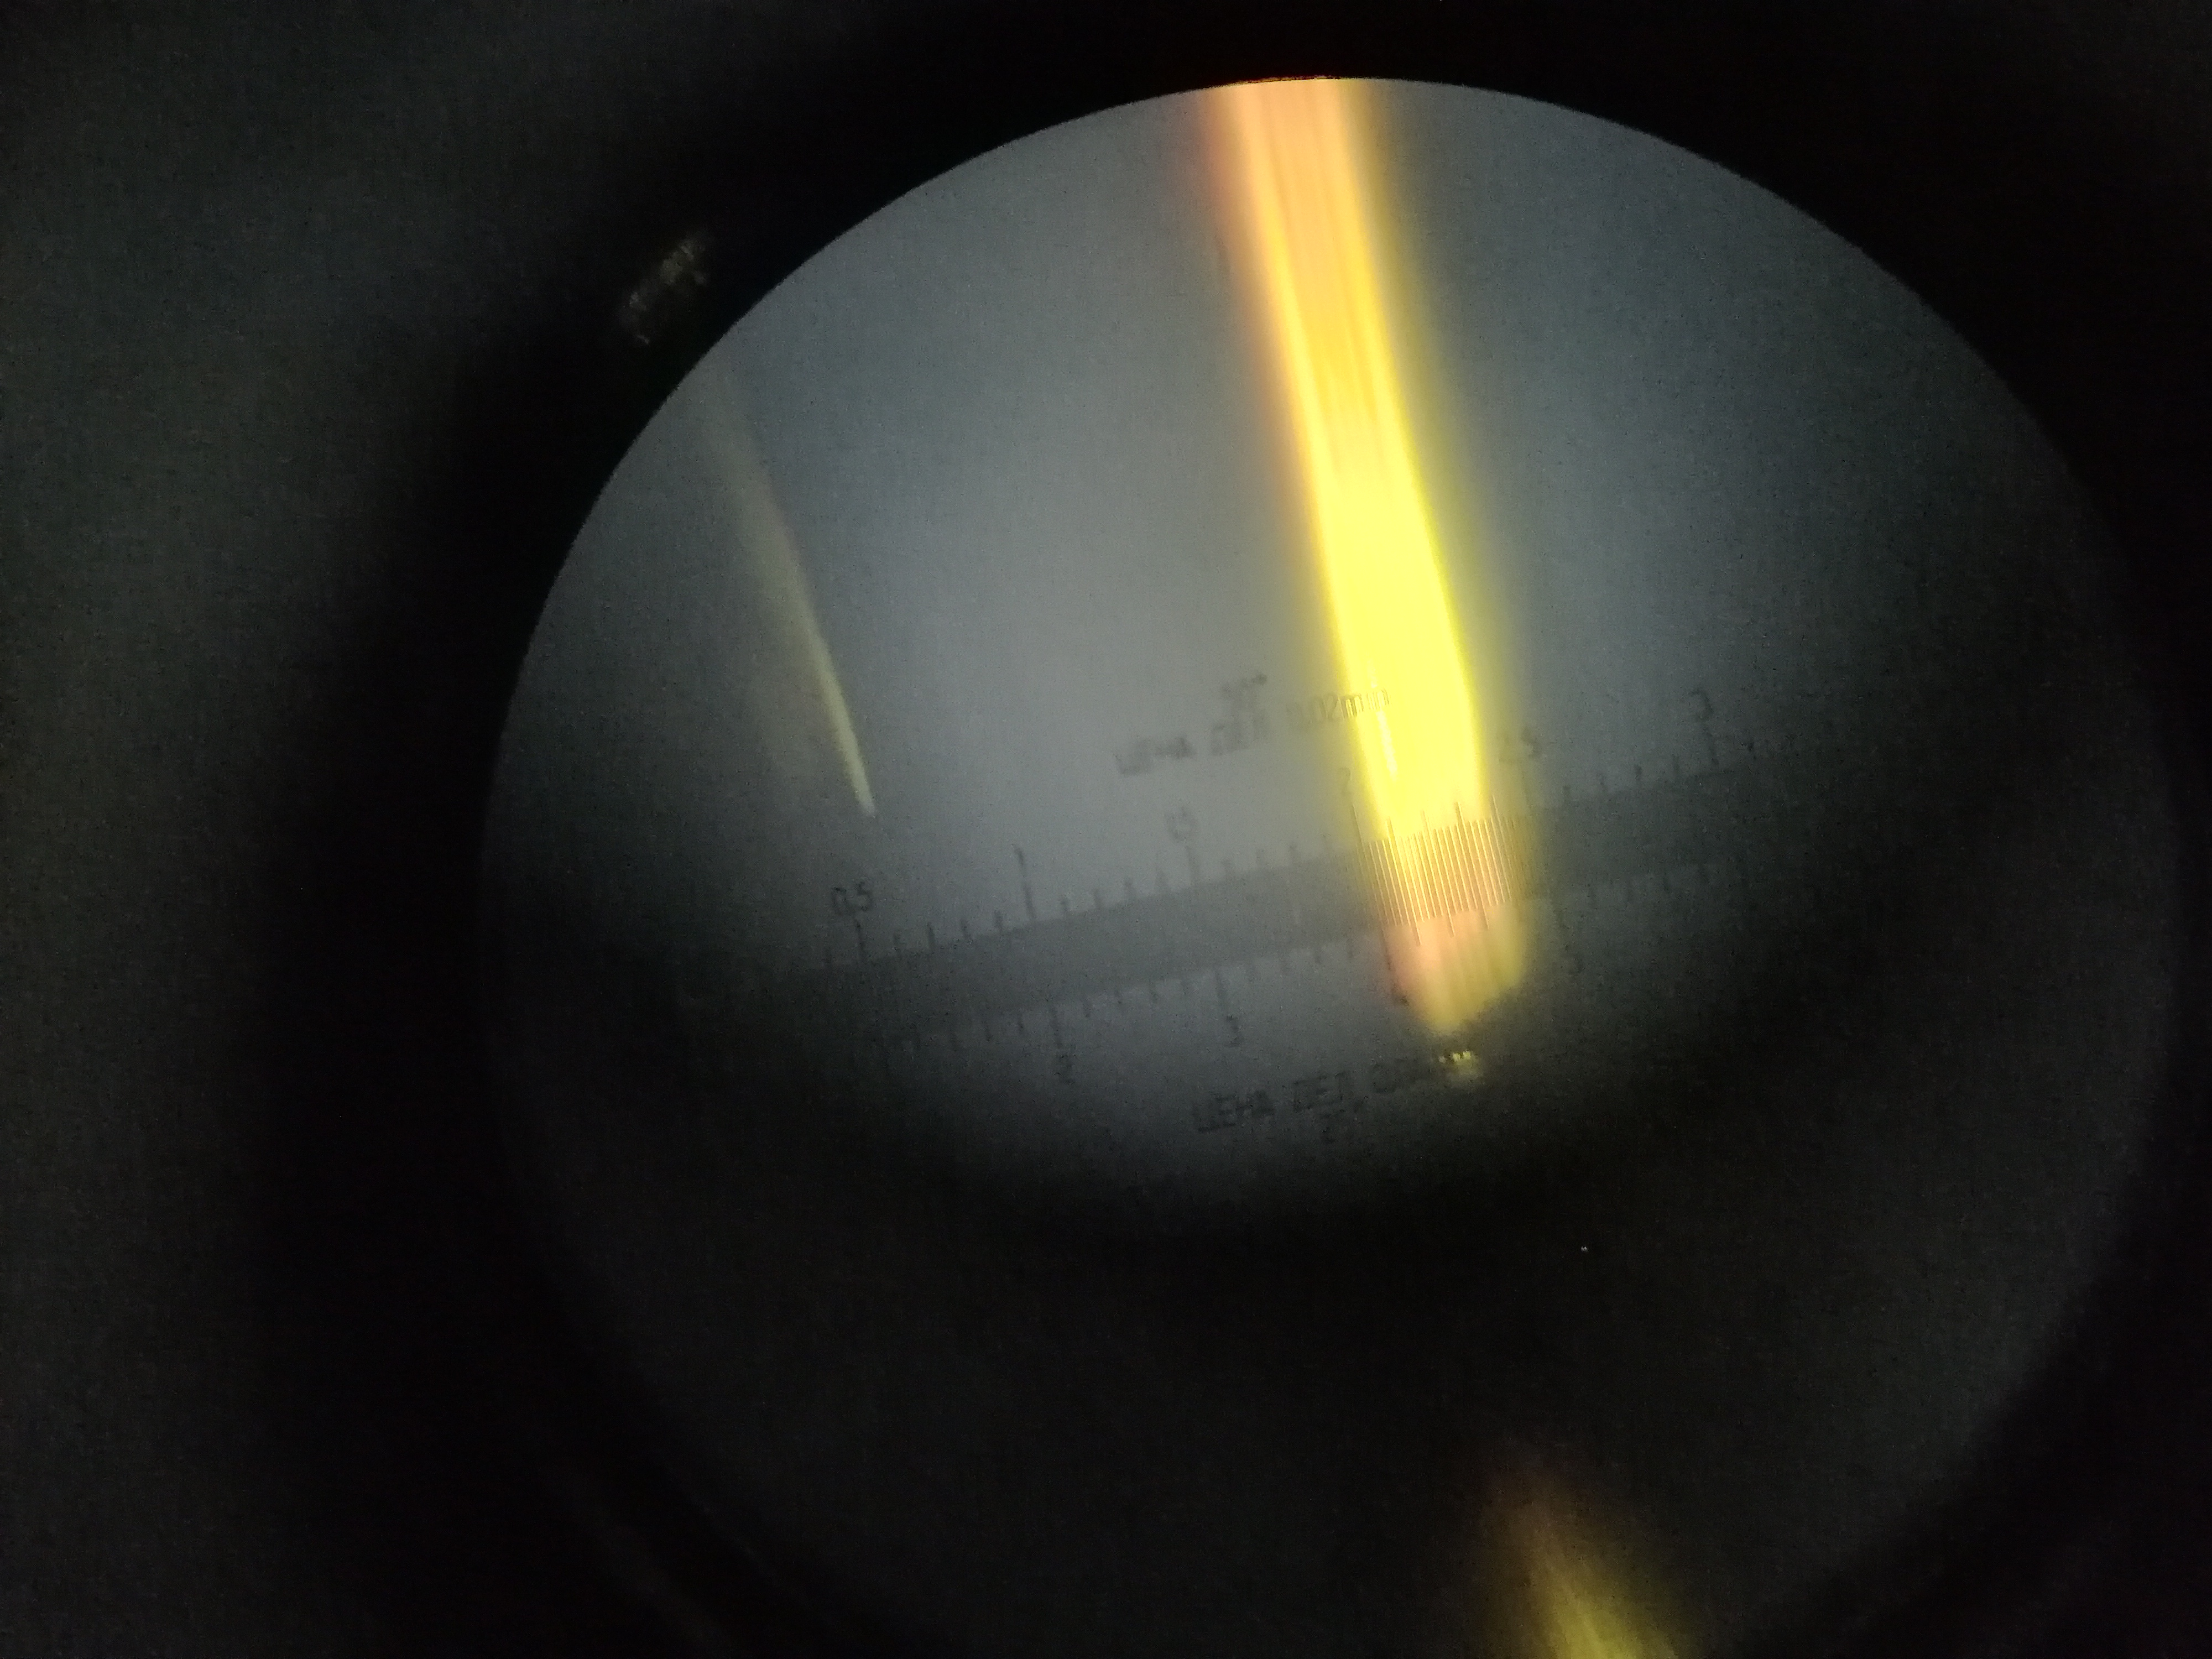
\includegraphics[width=1\textwidth]{frenel-4.jpg} \\ г) 4 полосы}
\end{minipage}
\begin{center}
\begin{minipage}{0.5\textwidth}
	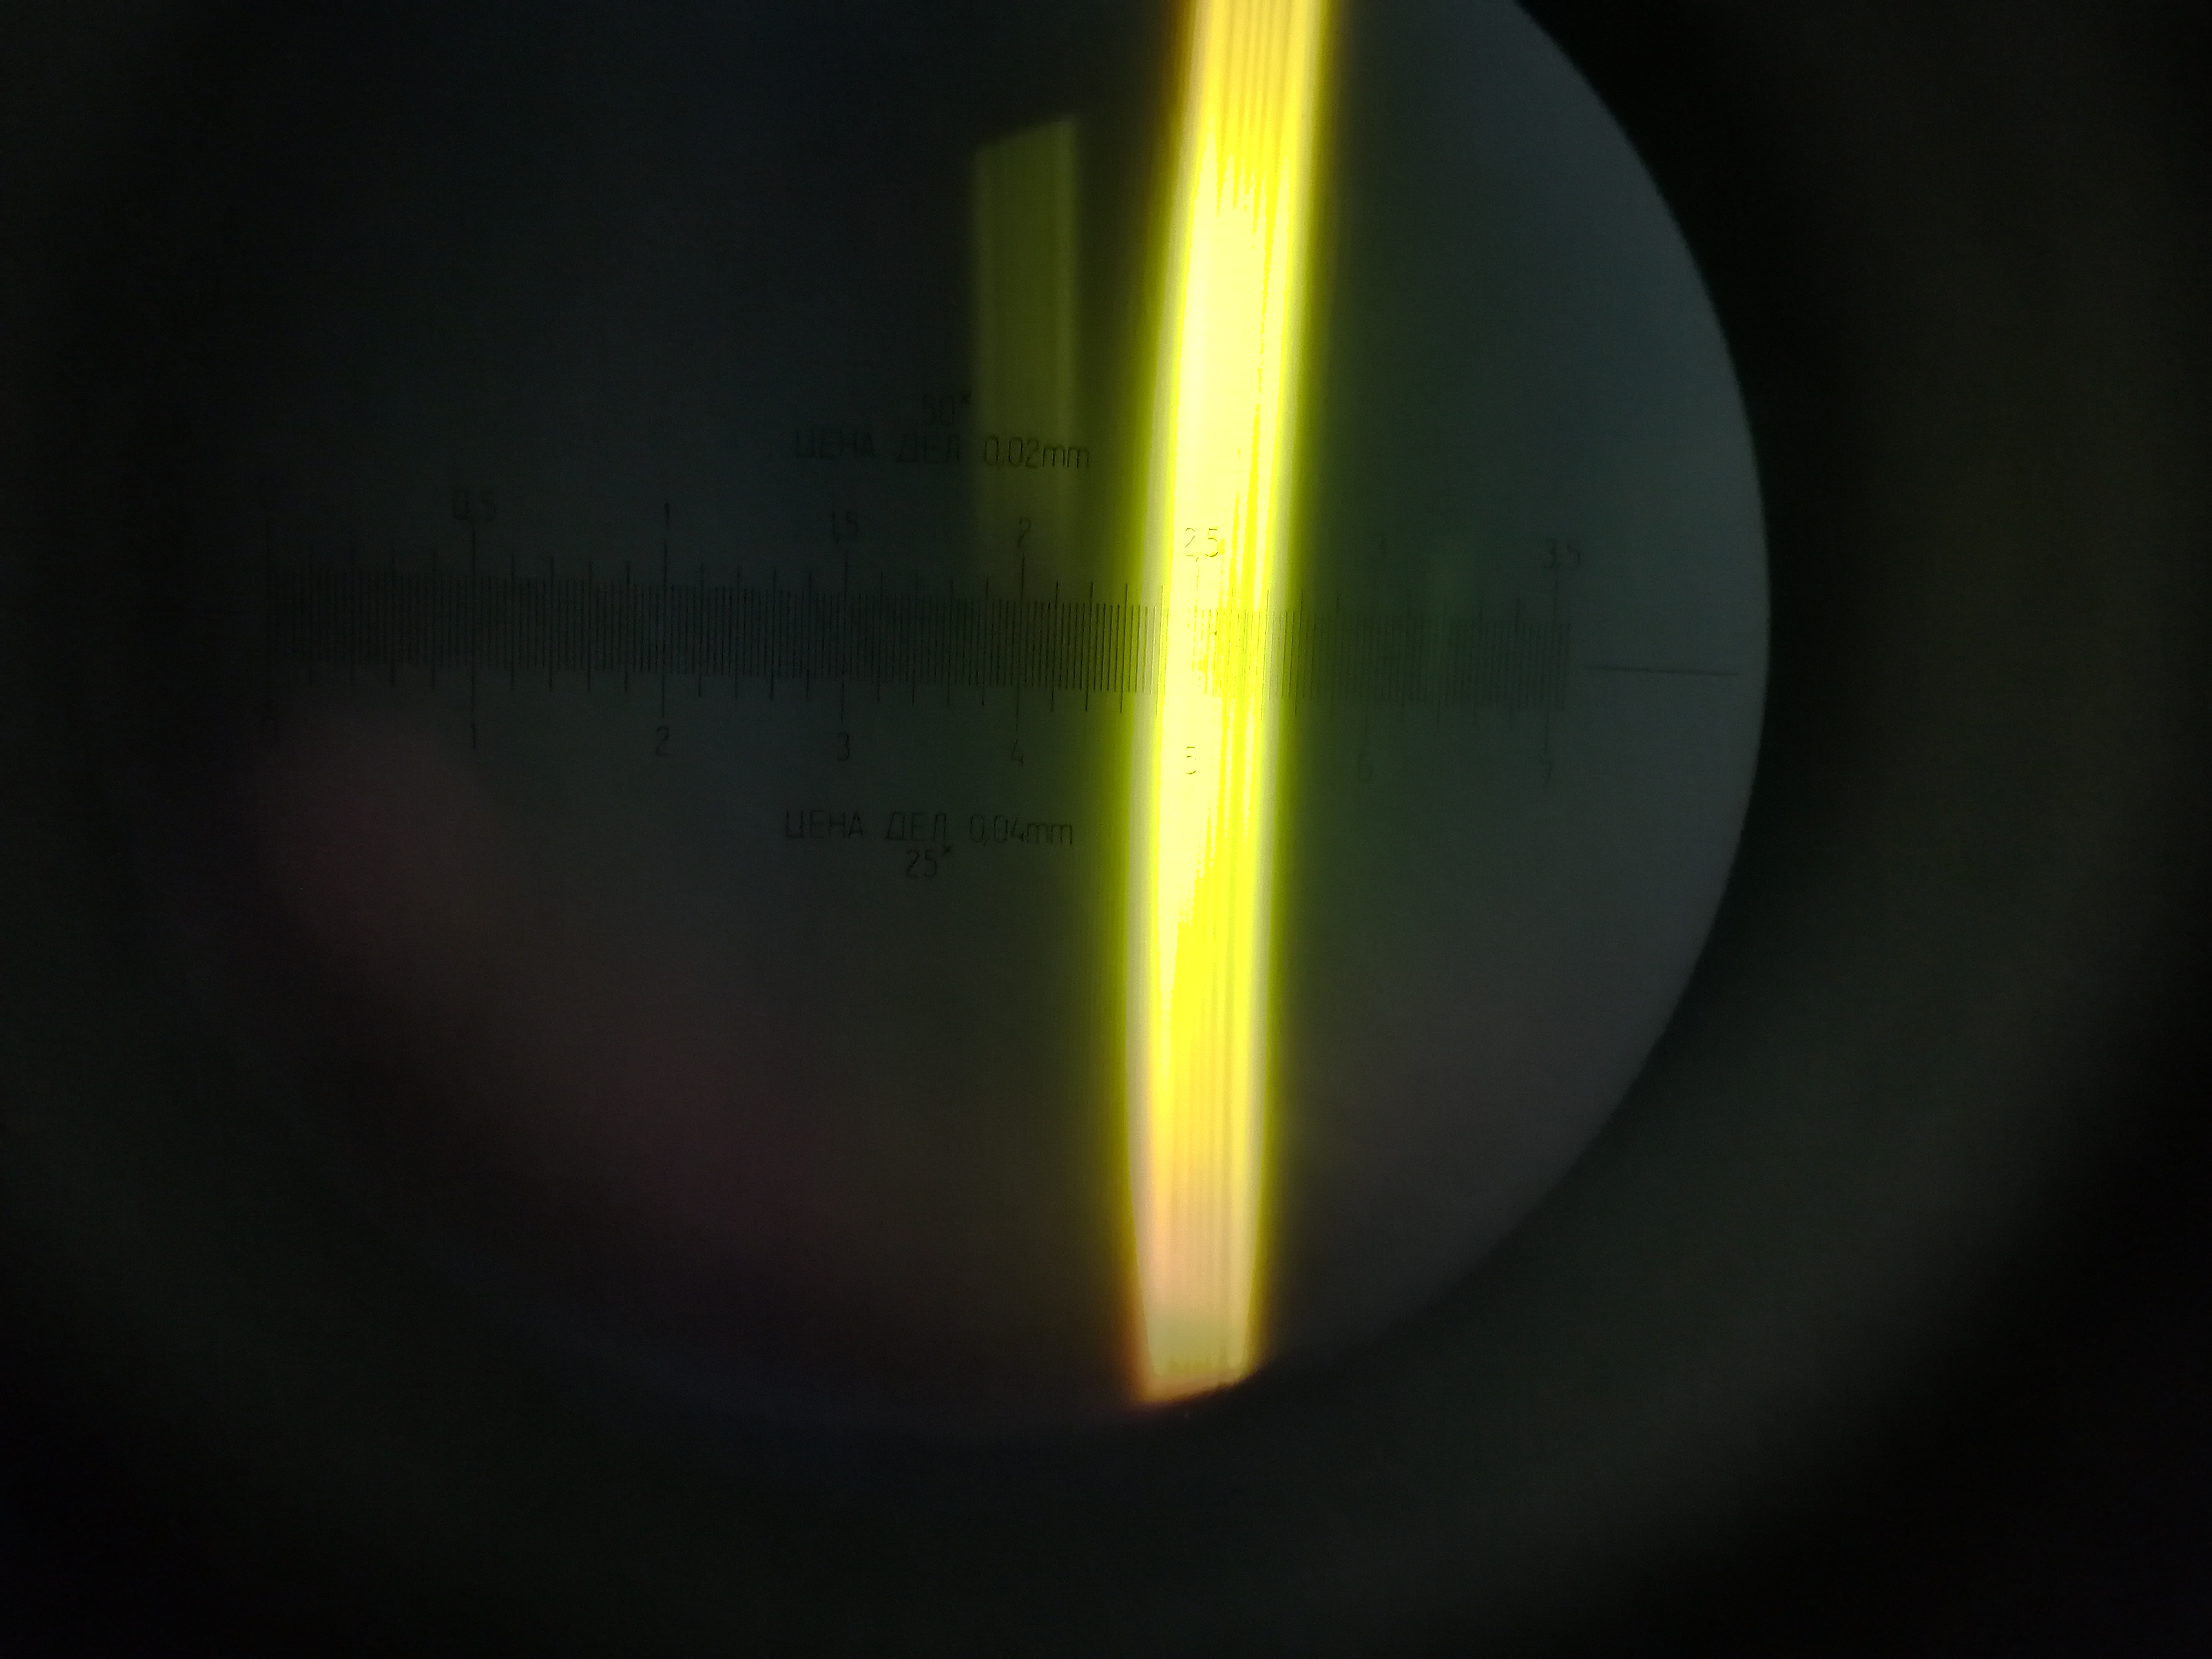
\includegraphics[width=1\textwidth]{frenel-5.jpg}
	\begin{center}
	\\ д) 5 полос
	\end{center}
\end{minipage}
\end{center}
\caption{Дифракция Френеля на щели}
\end{figure}

\newpage
	Сравним размер зон Френеля с измеренной шириной $b$ щели $S_2$, для этого рассчитаем $2 \xi_n$ по (\ref{Ширина зон}), где длина волны зеленой линии ртути $\lambda = $ 546,1 нм:

	\begin{center}
		\begin{tabular}{|c|c|c|c|c|c|}
			\hline
			$2\xi_n$, мкм & 229 & 273 & 292 & 296 & 296 \\ \hline
			$n$           & 1   & 2   & 3   & 4   & 5   \\ \hline
		\end{tabular}
	\end{center}

	\begin{figure}[h!]
		\begin{center}
		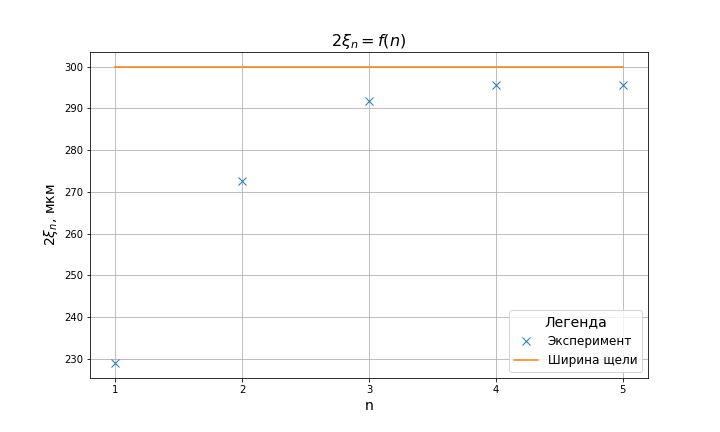
\includegraphics[width=1\textwidth]{graph1.png}
		\caption{Зависимость ширины френелевских зон от номера $n$}
		\label{График_ширина(номер)}
		\end{center}
	\end{figure}
	\item Измеренная ширина щели
	 \begin{itemize}
	 	\item по показаниям микрометрического винта: 0,302$~\pm~$0,005 мм;
		\item по показаниям микроскопа: 0,30$~\pm~$0,01 мм.
	 \end{itemize}

	 \clearpage
	 \item Снова сфокусируем микроскоп на щель. При небольшом удалении микроскопа от щели у её краев появляются узкие частые полосы (\textit{дифракция на краю экрана}).

	 \item Исследуем \textit{дифракцию Френеля на препятствии}: поставим вместо щели $S_2$ рамку с тонкой вертикальной нитью и настроим микроскоп на резкое изображение нити. При удалении микроскопа от нити на её фоне наблюдается чётное число тёмных дифракционных полос.

	 \begin{figure}[h!]
		 \begin{minipage}{0.5\textwidth}
			 \center{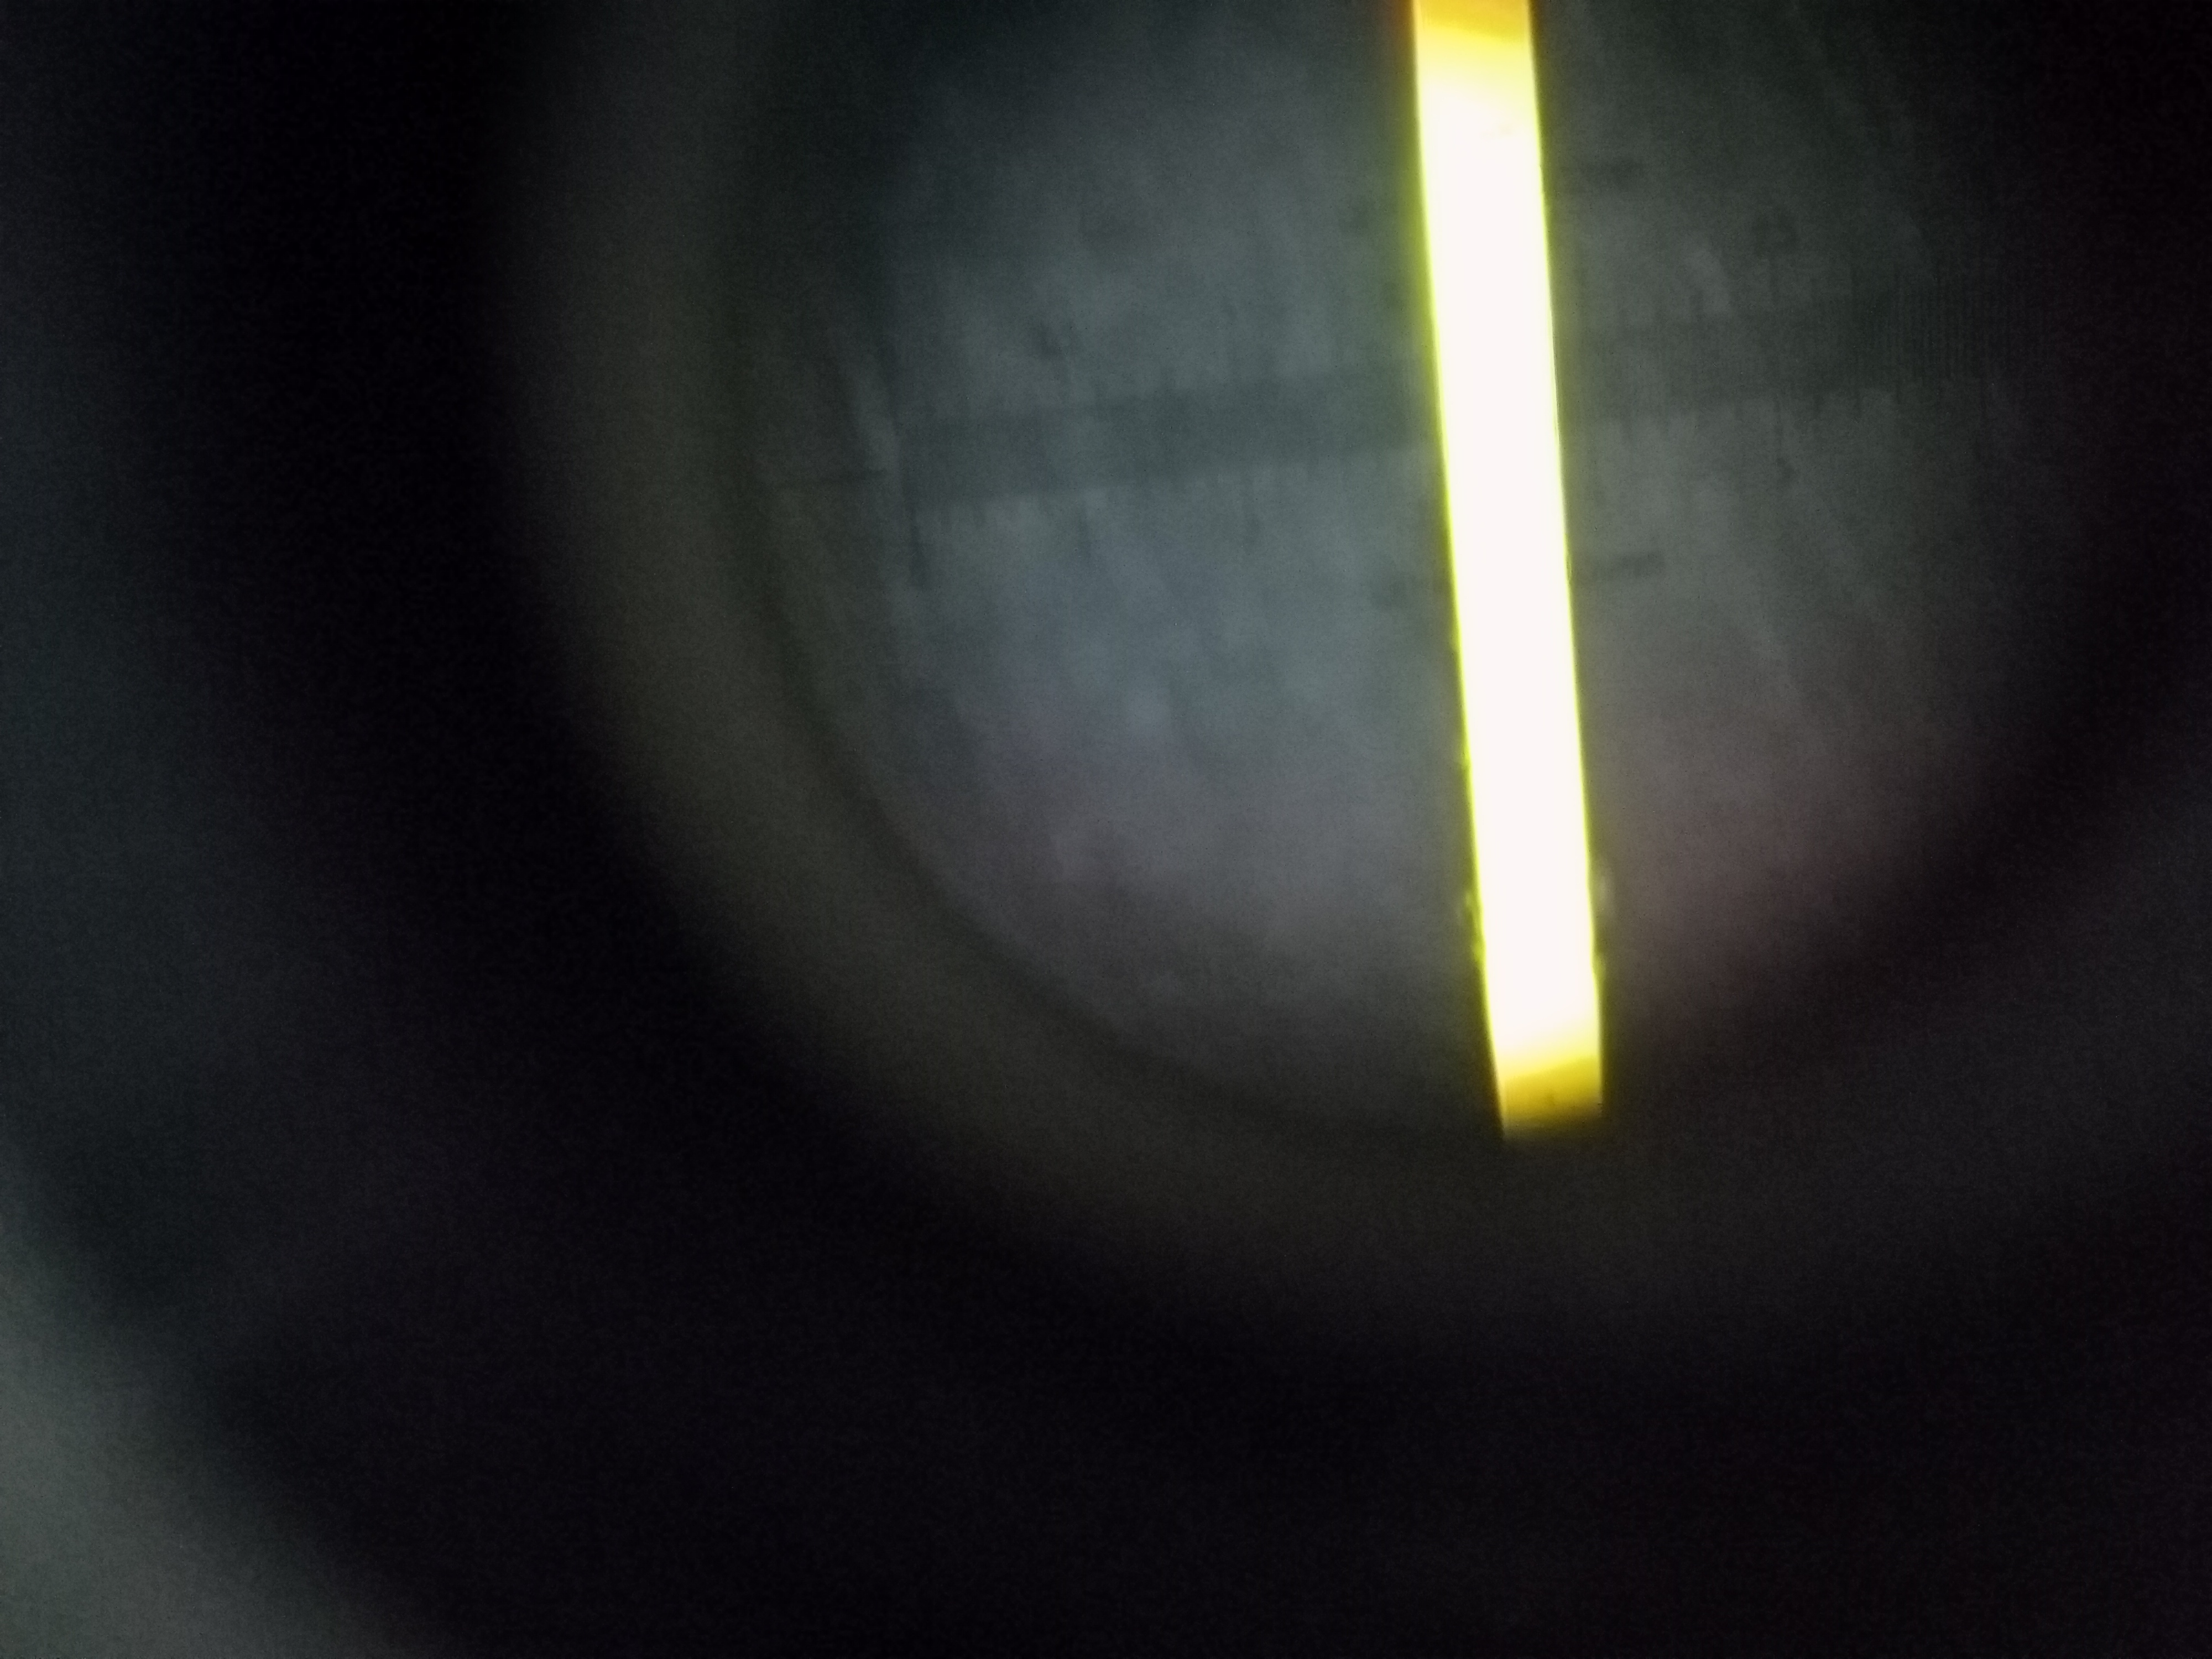
\includegraphics[width=1\textwidth]{frenel-edge.jpg}}
			 \caption{Дифракция Френеля на краю экрана}
		 \end{minipage}
		 \begin{minipage}{0.5\textwidth}
			 \center{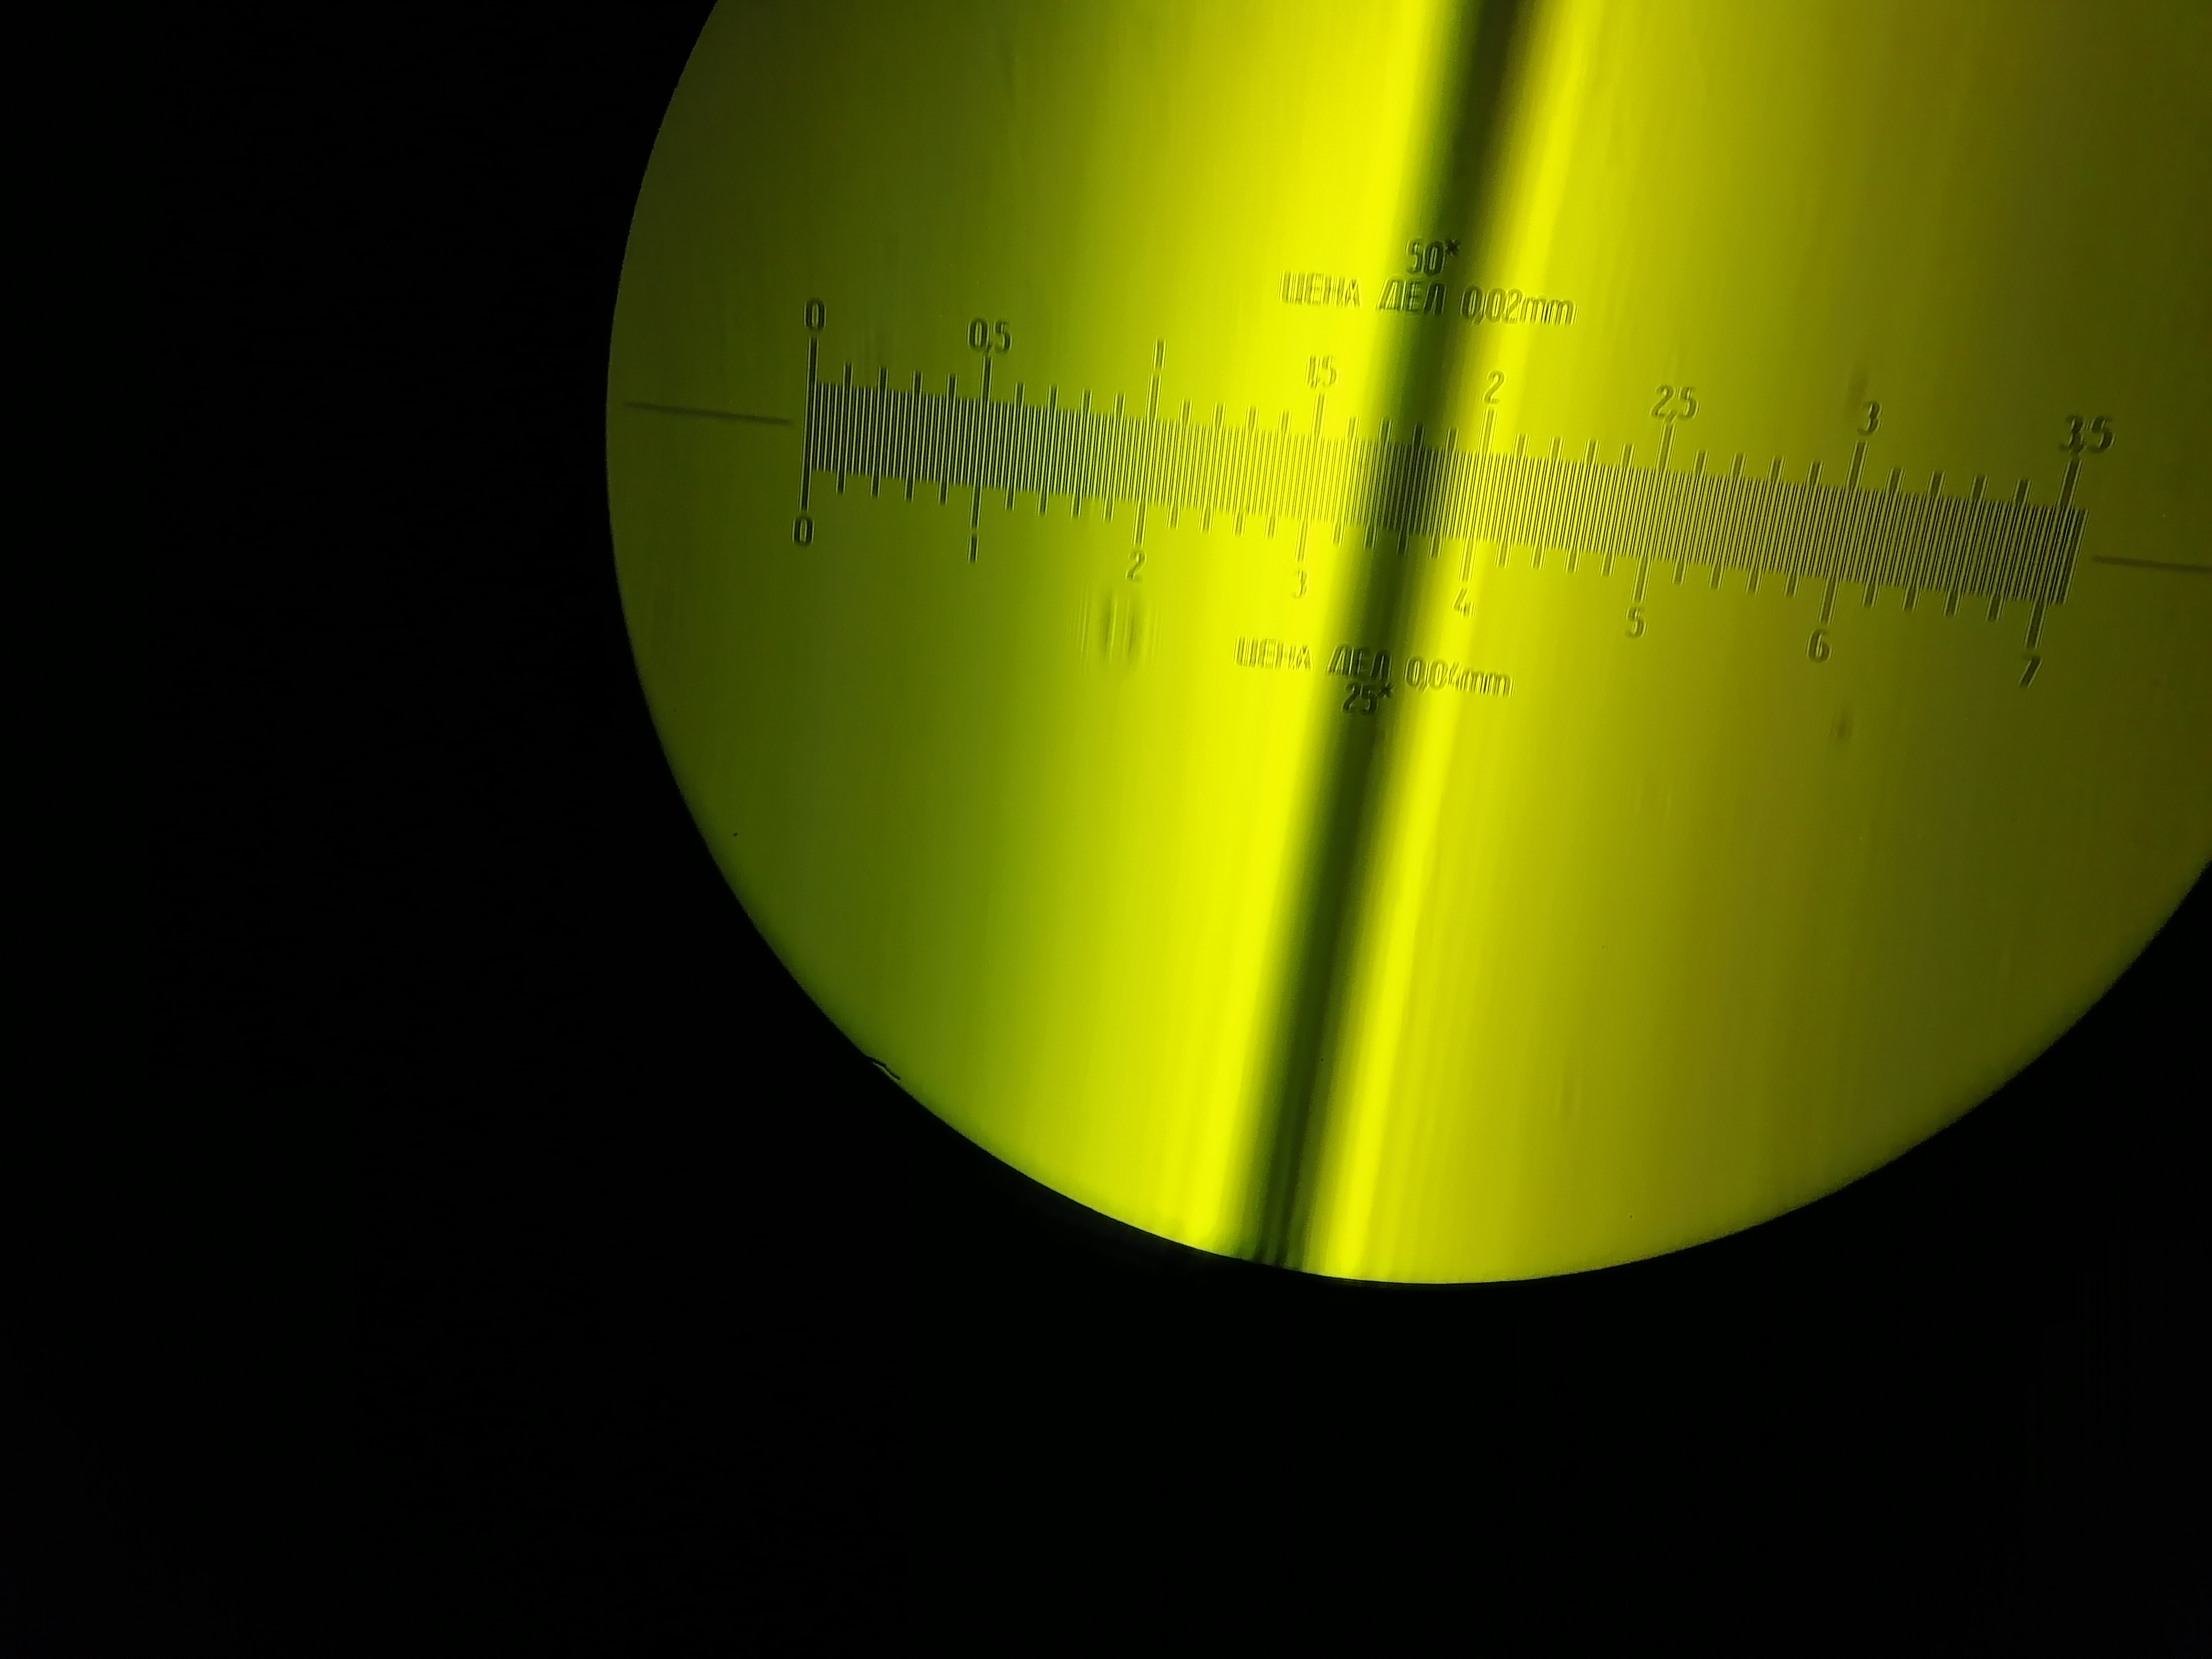
\includegraphics[width=1\textwidth]{frenel-barrier.jpg}}
	 	\caption{Дифракция Френеля на препятствии}
		\end{minipage}
	\end{figure}

	 \item Видимое число тёмных полос связано с шириной щели соотношением (\ref{Число Френеля}).

\end{enumerate}

\subsection{Дифракция Фраунгофера}

\begin{enumerate}
	\item Для перехода из ближней волновой зоны (дифракции Френеля) в дальнюю (Дифракция Фраунгофера) добавим к установке линзу $O_2$ (рис. \ref{Установка_Фраунгофер}). Фокусные расстояния линз $O_1$ и $O_2$ -- 10 см и 12,8 см соответственно. Ширина щели, определенная по микрометрическому винту -- 0,302$~\pm~$0,001 мм.

\clearpage
	\begin{figure}[h!]
	\begin{minipage}{1\textwidth}
		\center{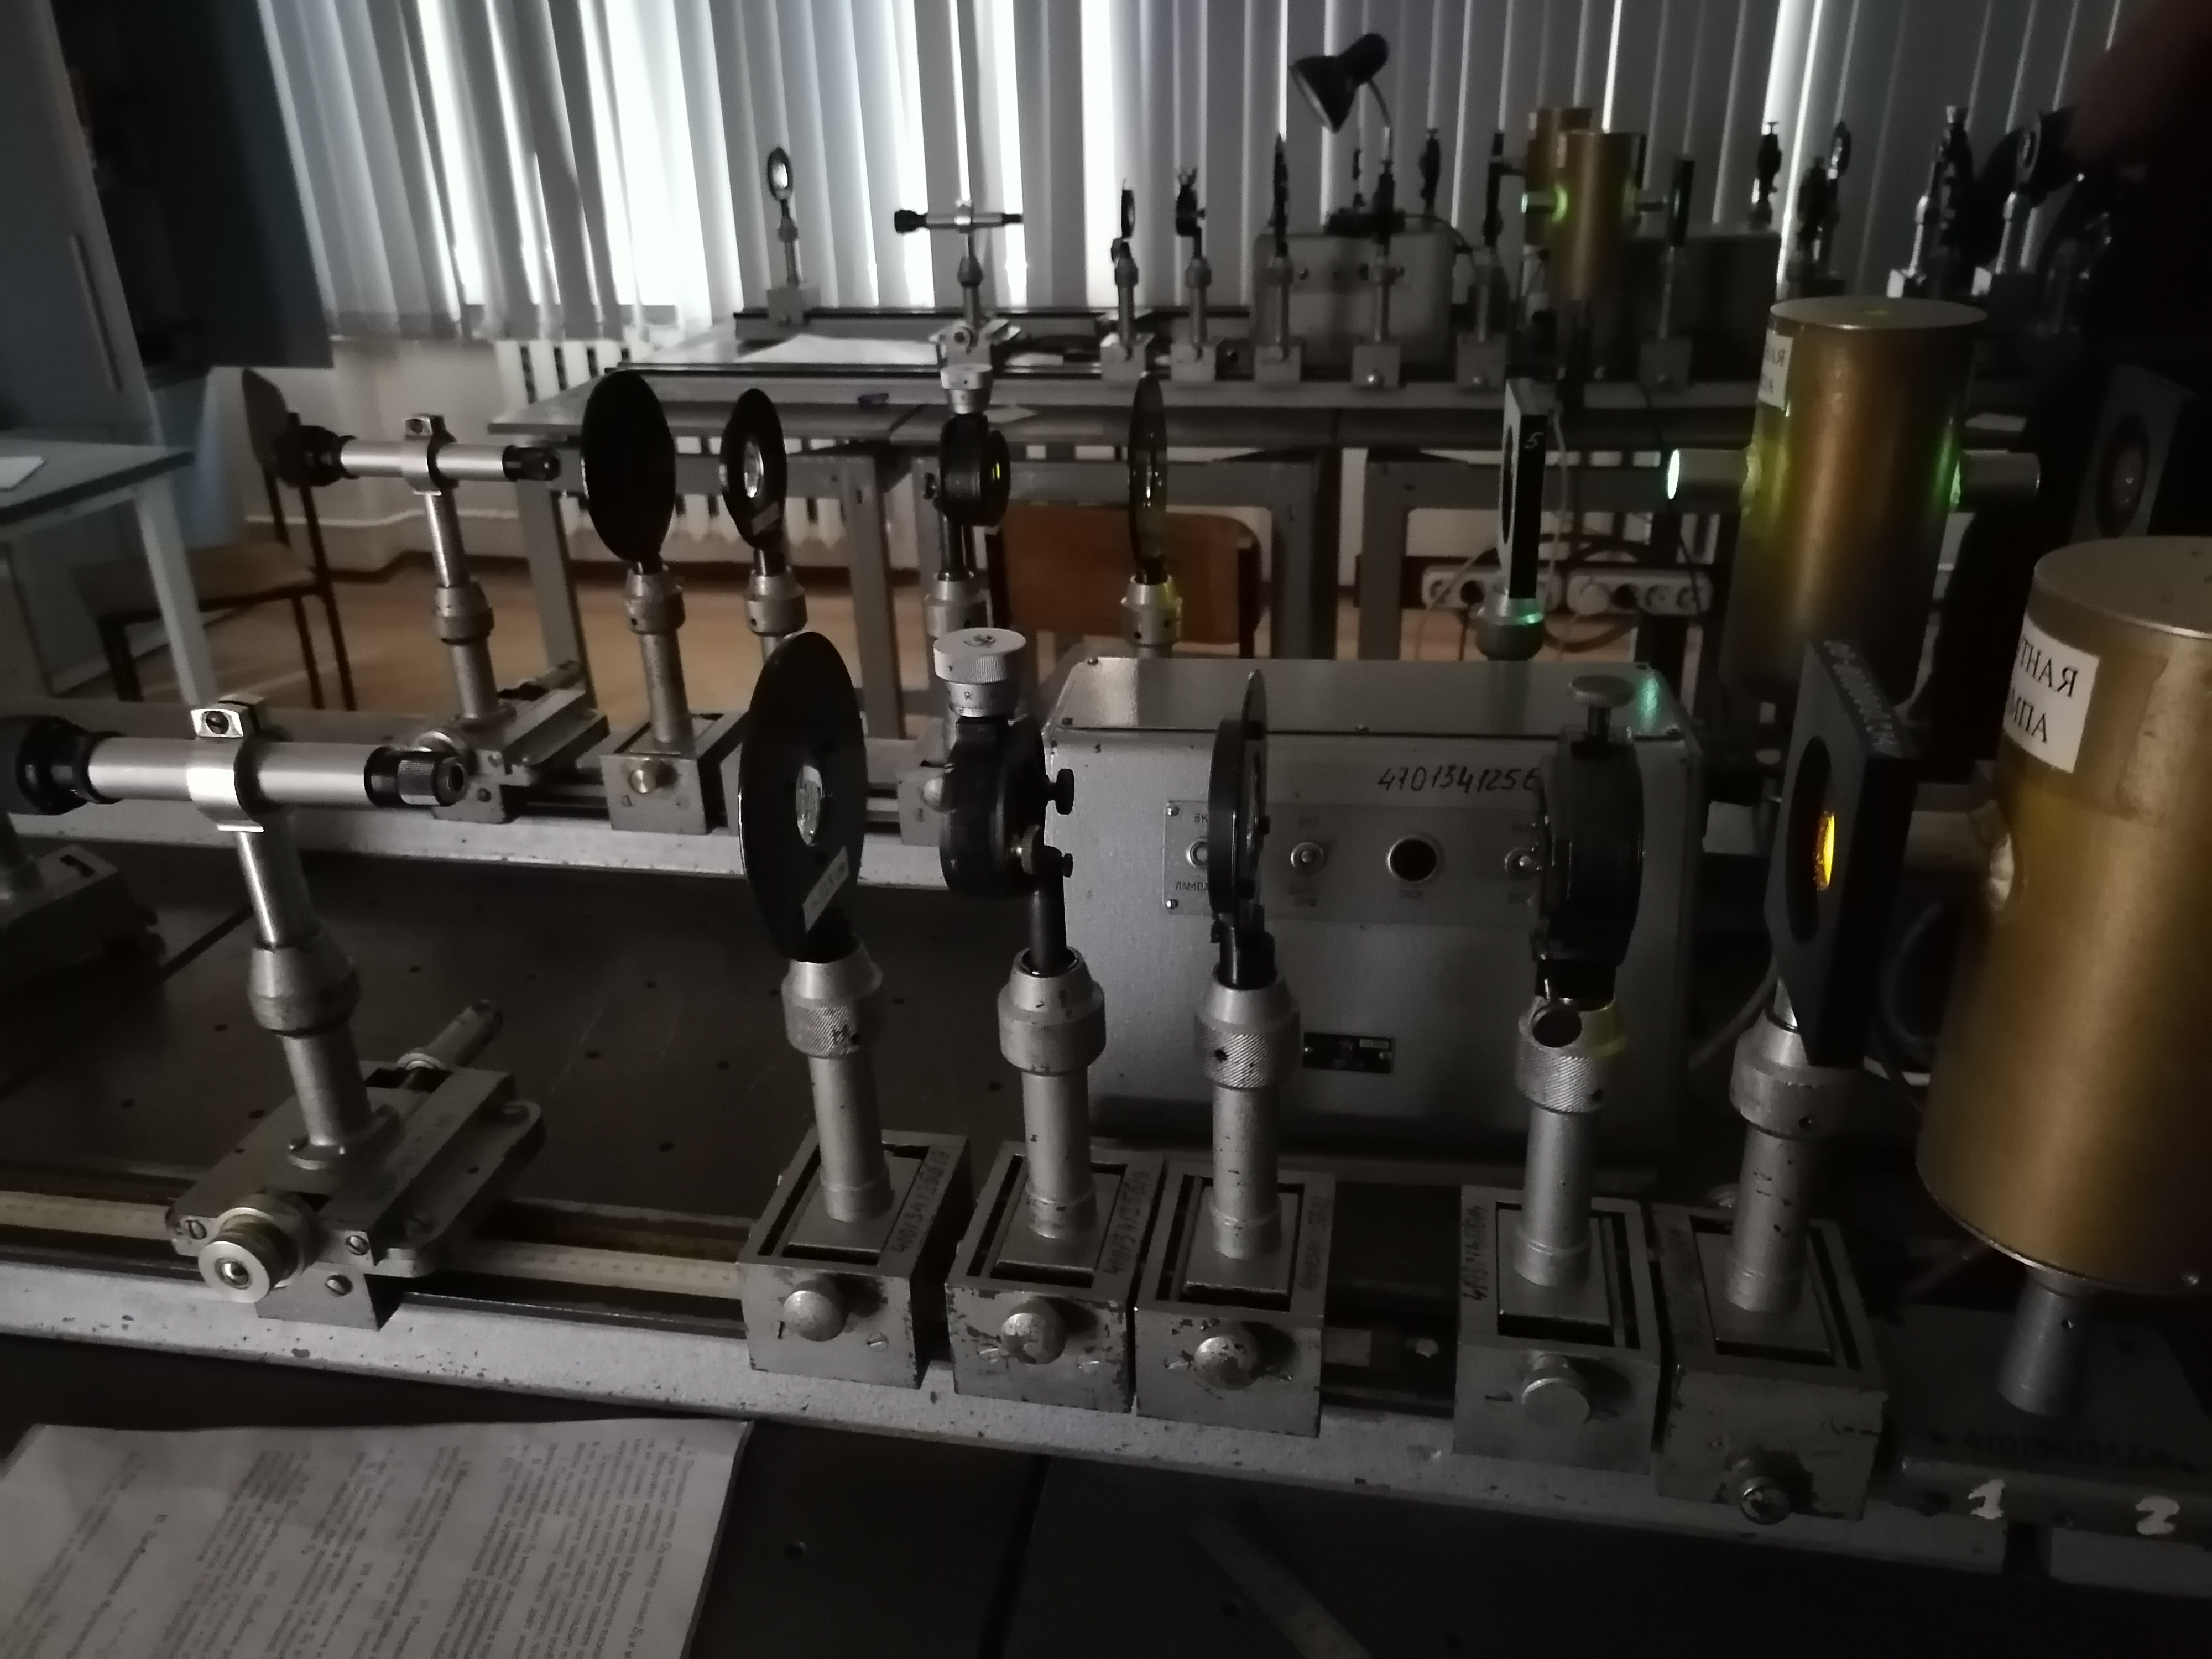
\includegraphics[width=0.8\textwidth]{facility_fraungofer.jpg}}
		\caption{Установка для наблюдения дифракции Фраунгофера}
	\end{minipage}
	\begin{minipage}{1\textwidth}
		\center{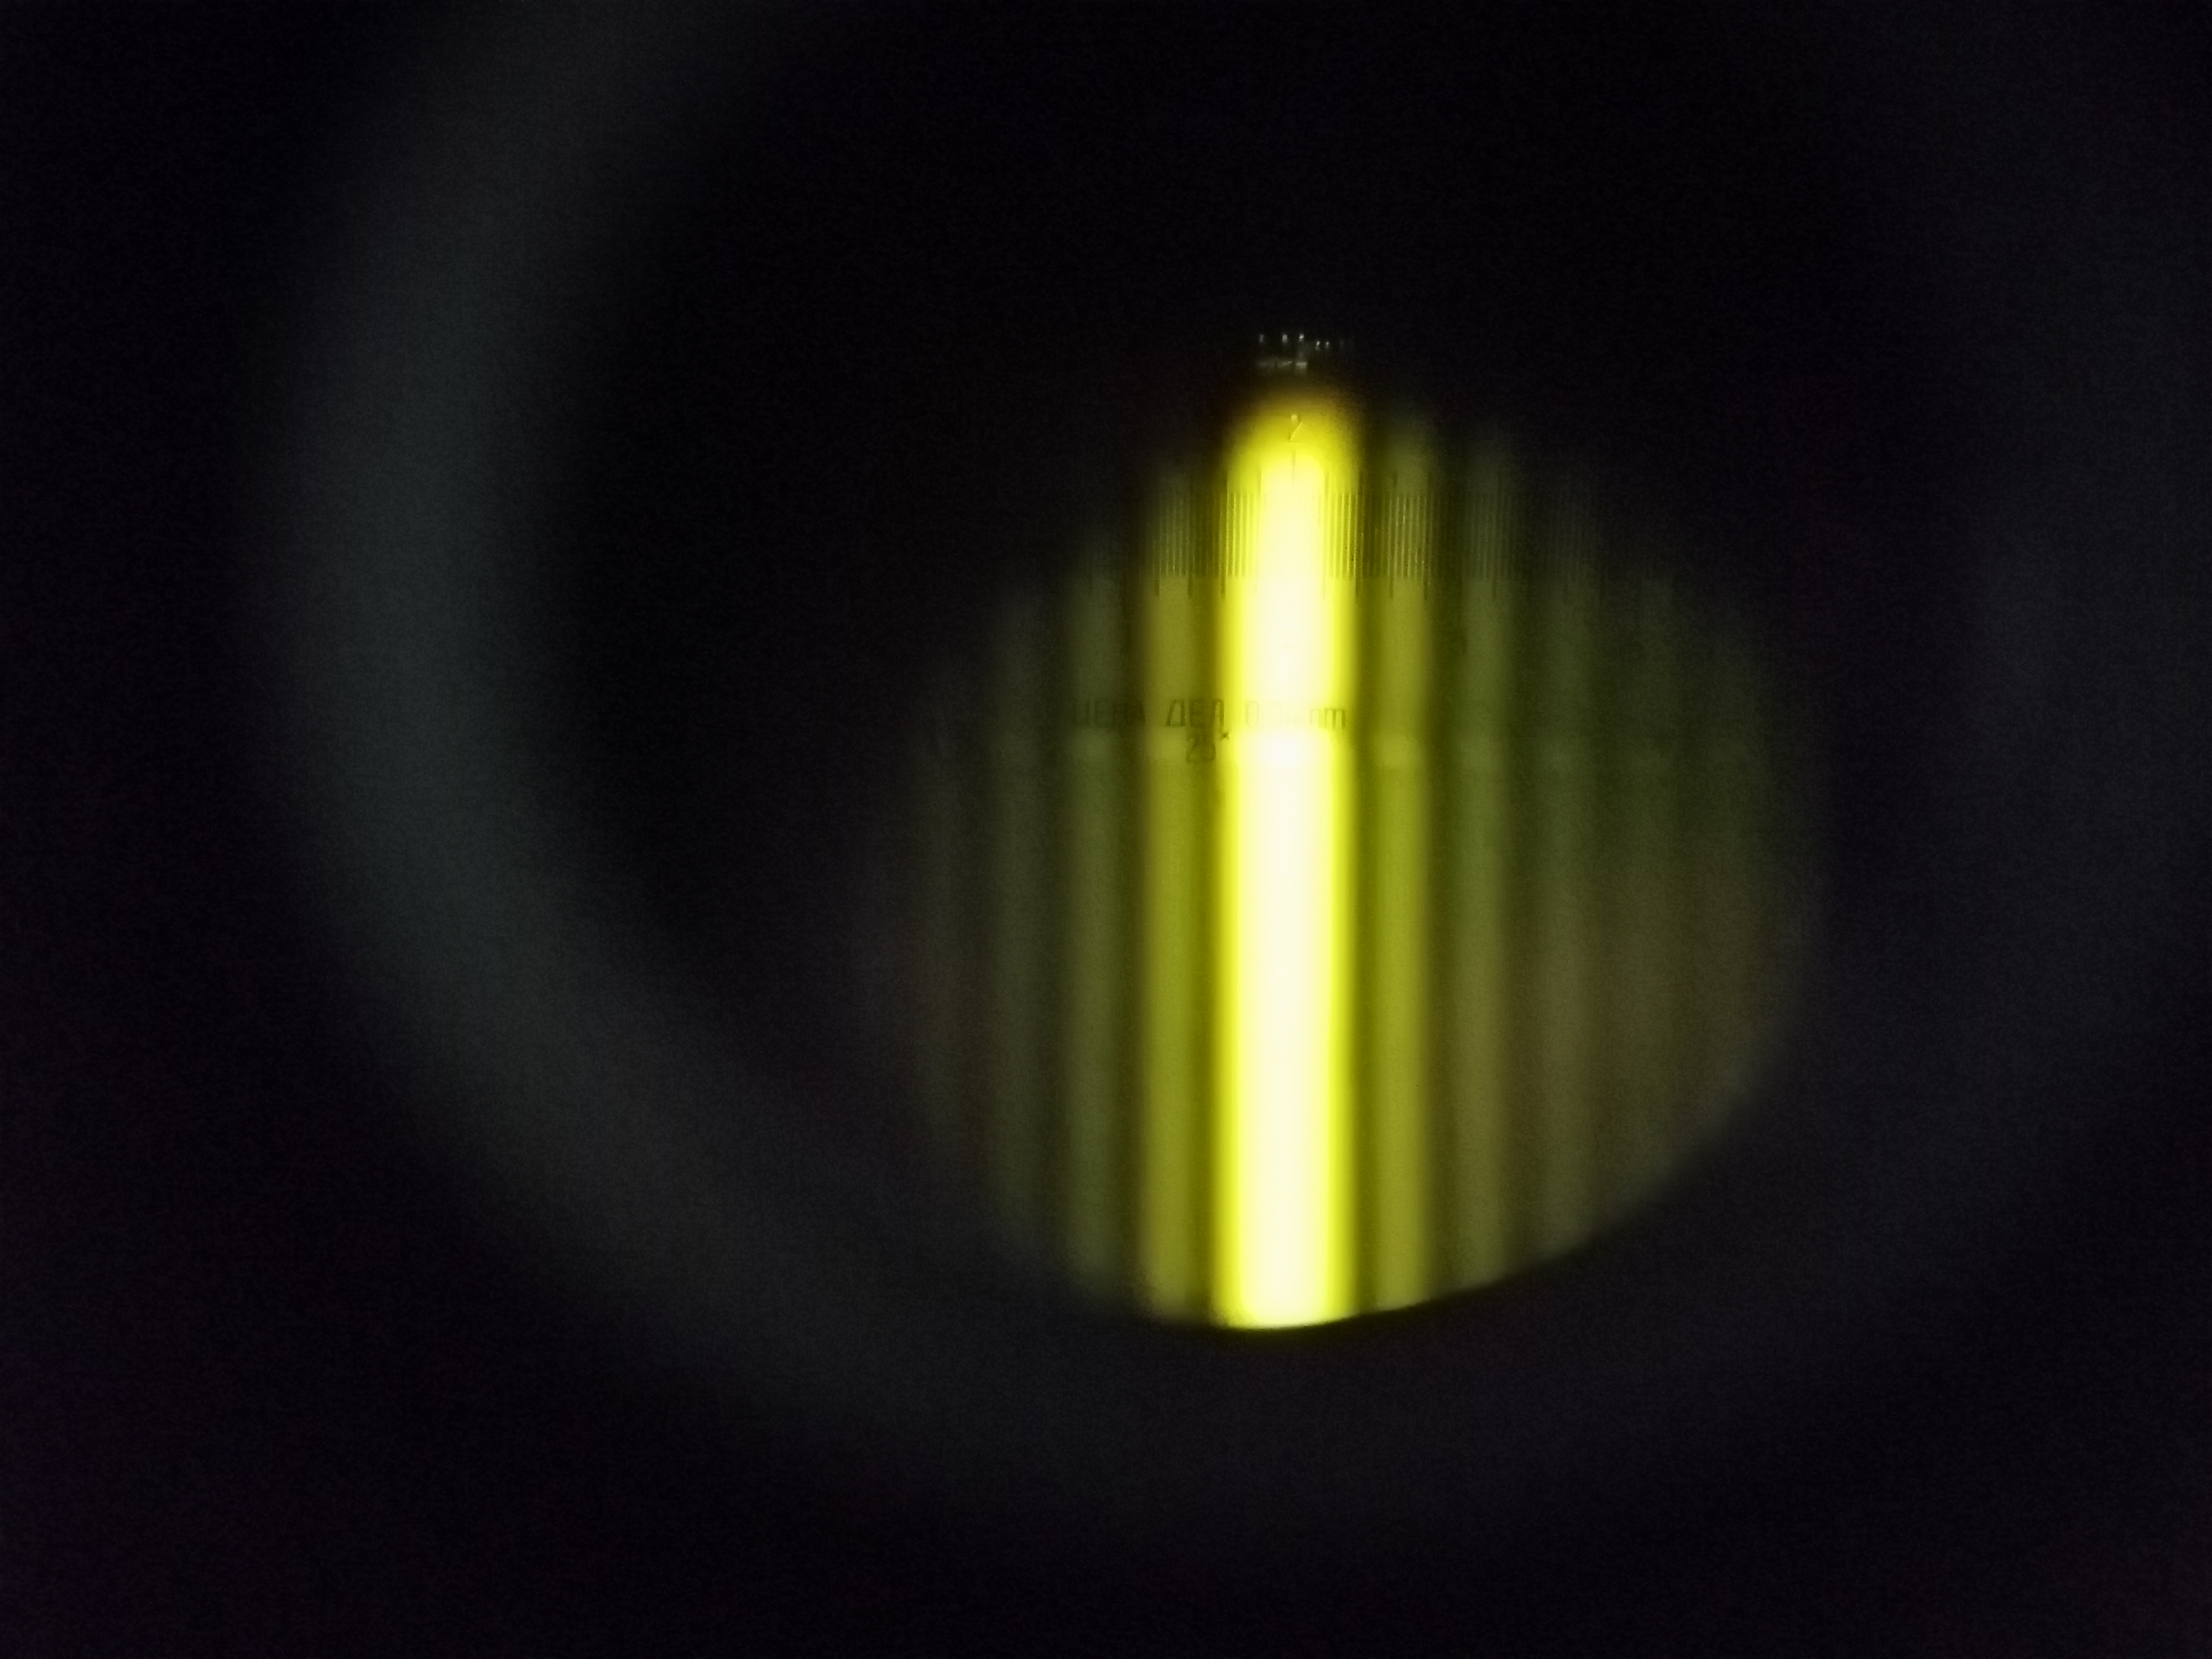
\includegraphics[width=0.8\textwidth]{fraungofer_difraction.jpg}}
		\caption{Картина дифракции Фраунгофера}
	\end{minipage}
	\end{figure}

	\item Измерим с помощью винта поперечного перемещения микроскопа координаты $X_m$ нескольких дифракционных минимумов (от $-m$ до $m$). Измерения проводились по шкале с ценой деления 0,02 мм.

	\begin{center}
		\begin{tabular}{|c|c|c|c|c|c|c|c|c|}
			\hline
			Деления   & 1,06 & 1,28 & 1,52 & 1,76 & 2,24 & 2,44 & 2,7 & 2,94 \\ \hline
			m         & -4   & -3   & -2   & -1   & 1    & 2    & 3   & 4    \\ \hline
			$X_m$, мкм & 21,2 & 25,6 & 30,4 & 35,2 & 44,8 & 48,8 & 54  & 58,8 \\ \hline
		\end{tabular}
	\end{center}

	\begin{figure}[h!]
		\begin{center}
		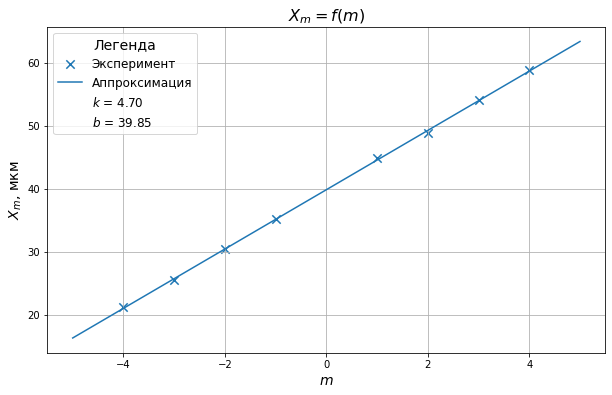
\includegraphics[width=1\textwidth]{graph2.png}
		\caption{Зависимость координаты минимума от его номера $m$}
		\end{center}
	\end{figure}

	По углу наклона прямой определим среднее среднее расстояние $\Delta X$ между соседними минимумами и рассчитаем ширину щели $b$ по формуле (\ref{Расстояние X_m}):

\[k = \Delta X = \dfrac{\lambda}{b}f_2~\Rightarrow~b=\dfrac{\lambda}{\Delta X}f_2\]

Таким образом ширина щели определенная:
\begin{itemize}
	\item Экспериментально по микрометрическому винту: 302$\pm$1 мкм;
	\item Из наклона графика: 297,5$\pm$ мкм
\end{itemize}

\end{enumerate}

\end{document}
